%% LyX 2.3.6.1 created this file.  For more info, see http://www.lyx.org/.
%% Do not edit unless you really know what you are doing.
\documentclass[english]{article}
\usepackage[T1]{fontenc}
\usepackage[latin9]{inputenc}
\usepackage{geometry}
\geometry{verbose,tmargin=3.5cm,bmargin=2.5cm,lmargin=2.5cm,rmargin=2.5cm,headsep=0.5cm,footskip=1cm}
\usepackage{float}
\usepackage{amsmath}
\usepackage{graphicx}

\makeatletter

%%%%%%%%%%%%%%%%%%%%%%%%%%%%%% LyX specific LaTeX commands.
\newcommand{\noun}[1]{\textsc{#1}}

\makeatother

\usepackage{babel}
\usepackage{listings}
\renewcommand{\lstlistingname}{Listing}

\begin{document}
\vspace*{\fill}
\noindent \begin{center}
\textbf{\emph{\noun{\huge{}EE2703: Applied Programming Lab}}}{\huge\par}
\par\end{center}

\begin{center}
\textbf{\emph{\noun{\huge{}Week 9: Spectra of Non-Periodic Signals}}}{\huge\par}
\par\end{center}

\begin{center}
{\Large{}Author: Surya Prasad S, EE19B121}{\Large\par}
\par\end{center}

\begin{center}
{\Large{}May 22nd, 2021}{\Large\par}
\par\end{center}

\begin{center}
{\Large{}\vspace*{\fill}\pagebreak}{\Large\par}
\par\end{center}

\section{{\LARGE{}Abstract:}}
\noindent \begin{flushleft}
{\large{}In last week's assignment, we had analysed periodic functions.
This week we shall analyse non-periodic signals and minimise the errors
that arise from Gibbs phenomenon. We shall also use a techinique called
Hamming Windowing to reduce the errors.}{\large\par}
\par\end{flushleft}

\section{{\LARGE{}Code and Plot Analysis:}}

\subsection{Libraries imported:}

{\large{}}
\begin{lstlisting}[language=Python]
from pylab import *
\end{lstlisting}
{\large\par}

\subsection{Common Function to perform FFT:}

{\large{}}
\begin{lstlisting}[language=Python,breaklines=true]
def plot_FFT(func, TITLE, r = [-pi, pi], N = 64, xlimit = 10, odd_signal = False, indB = False, estimate_flag = False):
    ## Time vector is being declared. Here we remove the last point because it will overlap with the initial point
    t = linspace(r[0], r[1], N + 1)[:-1]

    ## Frequency vector is being declared. temp is a just a temporary variable for the purpose of calculation
    temp = N * (pi/(r[1] - r[0]))
    w = linspace(-temp, temp, N + 1)[:-1]

    ## Computing functional values in the time domain and frequency domain
    ### For odd signals we make y[0] as 0 to reduce the error
    y = func(t)

    if odd_signal:
        y[0] = 0

    Y = fftshift(fft(fftshift(y)))/float(N)

    ## Plotting phase and magnitude plots for DFT of the signals
    figure()

    if indB:
        subplot(2, 1, 1)
        title("Frequency Spectrum of " + TITLE)
        semilogx(w, 20 * log10(abs(Y)), lw = 2)
        xlim([1, 10])
        ylim([-20, 0])
        ylabel(r"$|Y|$ (in dB)", size = 16)
        grid(True)

    else:
        subplot(2, 1, 1)
        title("Frequency Spectrum of " + TITLE)
        plot(w, abs(Y), lw = 2)
        xlim([-xlimit, xlimit])
        ylabel(r"$|Y|$", size = 16)
        grid(True)

    subplot(2, 1, 2)
    ii = where(abs(Y) > 1e-3)
    scatter(w, angle(Y), marker = 'o', color = '#D9D9D9')
    plot(w[ii], angle(Y[ii]), 'go', lw = 2)
    xlim([-xlimit, xlimit])
    ylabel(r"$\angle$$Y$ (in rad)", size = 16)
    xlabel(r"$\omega$ (in rad/s)", size = 16)
    grid(True)

    show()

    if estimate_flag:
    	return w, abs(Y), angle(Y)
\end{lstlisting}
{\large\par}

\subsection{DFT Analysis of $sin(\sqrt{2}t)$:}
\noindent \begin{flushleft}
{\large{}Let's try to find the DFT of the sinusoid. }{\large\par}
\par\end{flushleft}

\noindent {\large{}
\[
Y[k]=-2j\sum_{n=0}^{\frac{N}{2}-1}y[n]sin(\frac{2\pi kn}{N})+(-1)^{k}y[\frac{N}{2}]
\]
}{\large\par}
\begin{center}
{\large{}$y[0]=0$}{\large\par}
\par\end{center}

\noindent \begin{flushleft}
{\large{}For $i\in{1,2,....,\frac{N}{2}-1}$}{\large\par}
\par\end{flushleft}

\begin{center}
{\large{}$y[i]=-y[N-i]$}{\large\par}
\par\end{center}

\begin{center}
{\large{}$y[\frac{N}{2}]=sin(t_{\frac{N}{2}})=sin(-t_{max})$}{\large\par}
\par\end{center}

\noindent {\large{}
\[
Y[k]=\sum_{n=0}^{\frac{N}{2}-1}y[n](exp(j\frac{2\pi kn}{N})-exp(-j\frac{2\pi kn}{N}))+y[\frac{N}{2}]exp(j\pi k)
\]
}{\large\par}

\noindent {\large{}
\[
Y[k]=-2j\sum_{n=0}^{\frac{N}{2}-1}y[n]sin(\frac{2\pi kn}{N})+(-1)^{k}y[\frac{N}{2}]
\]
}{\large\par}
\noindent \begin{flushleft}
{\large{}We can see that the DFT is not completely imaginary even
though the CTFT is purely imaginary. Hence we shall make $y[0]$ to
be 0. Using this result, let's plot the Frequency Spectrum of $sin(\sqrt{2}t)$.}{\large\par}
\par\end{flushleft}

{\large{}}
\begin{figure}[H]
\begin{centering}
{\large{}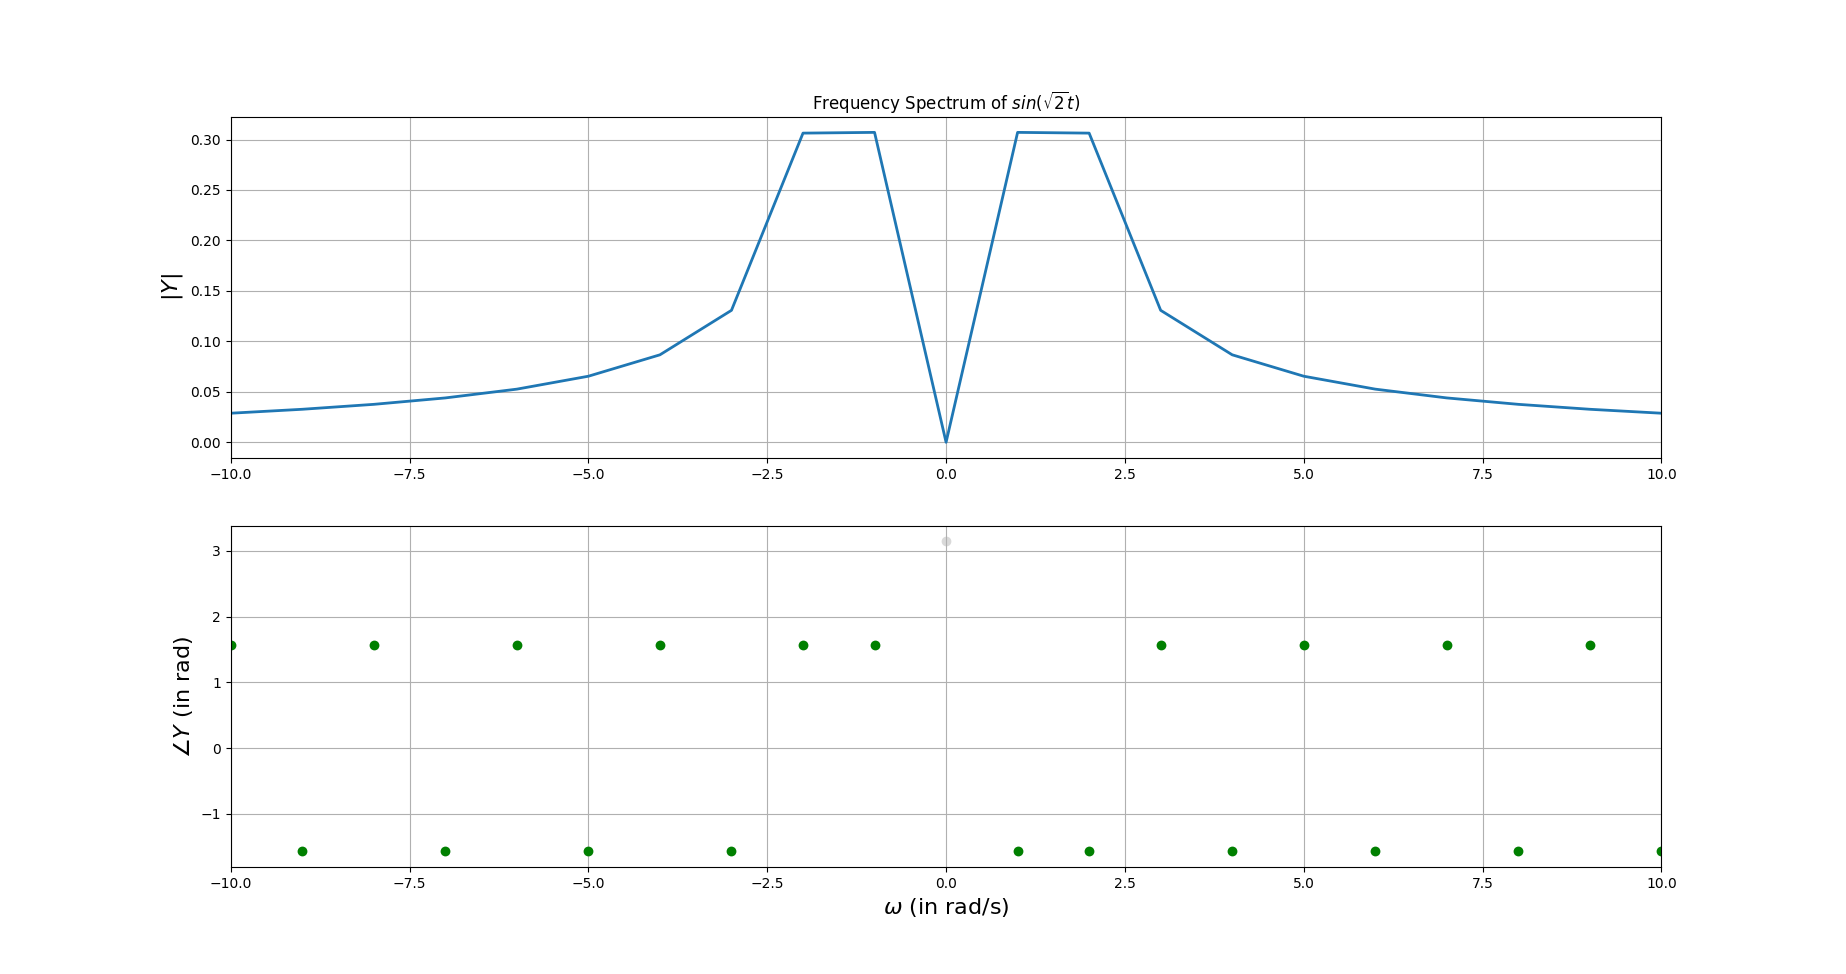
\includegraphics[scale=0.3]{Figure_1}}{\large\par}
\par\end{centering}
{\large{}\caption{{\large{}Frequency Spectrum of $sin(\sqrt{2}t)$ sampled 64 times}}
}{\large\par}

\end{figure}
{\large\par}
\noindent \begin{flushleft}
{\large{}As we can see in the plot instead of two peaks at $\pm\sqrt{2}$,
we got two peaks each with two values and a gradually decaying magnitude.
The phase plot is as expected. If we look at the region we have sampled,
and construct a periodic function with it we get the following plots:}{\large\par}
\par\end{flushleft}

{\large{}}
\begin{figure}[H]
\begin{centering}
{\large{}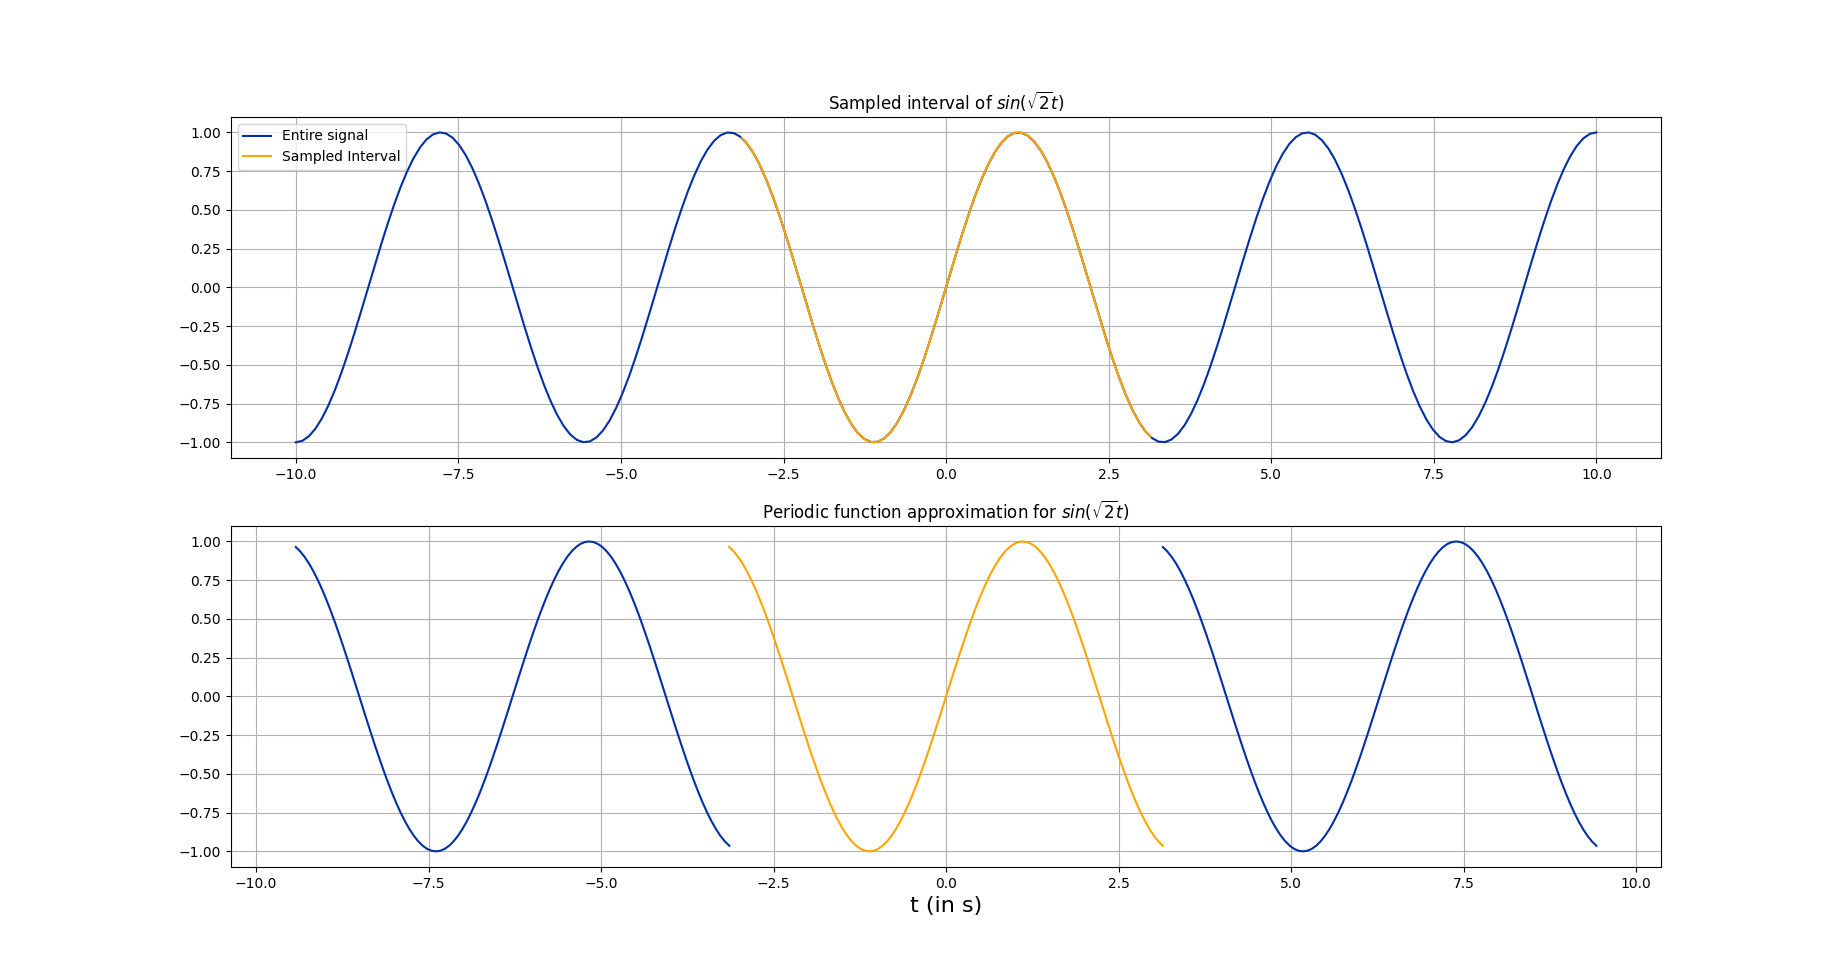
\includegraphics[scale=0.3]{Figure_1_2}}{\large\par}
\par\end{centering}
{\large{}\caption{{\large{}Periodic plot of sampled interval}}
}{\large\par}

\end{figure}
{\large\par}
\noindent \begin{flushleft}
{\large{}The plot is discontinous. This leads to a large number of
errors because of Gibbs phenomenon. Hence we see significant magnitudes
at higher frequencies. }{\large\par}
\par\end{flushleft}

\pagebreak{}
\noindent \begin{flushleft}
{\large{}Let's try to understand this concept by analysing the unit
ramp function.}{\large\par}
\par\end{flushleft}

\begin{center}
{\large{}$f(t)=t,-\pi<t<\pi$}{\large\par}
\par\end{center}

\noindent \begin{flushleft}
{\large{}The Fourier series of this ramp is }{\large\par}
\par\end{flushleft}

\begin{center}
{\large{}$f(t)=2(\frac{sint}{1}-\frac{sin2t}{2}+\frac{sin3t}{3}-\ldots)$}{\large\par}
\par\end{center}

\noindent \begin{flushleft}
{\large{}So here the coefficients are expected to decay very slowly.
Let's plot the magnitude response for the ramp function.}{\large\par}
\par\end{flushleft}

{\large{}}
\begin{figure}[H]
\begin{centering}
{\large{}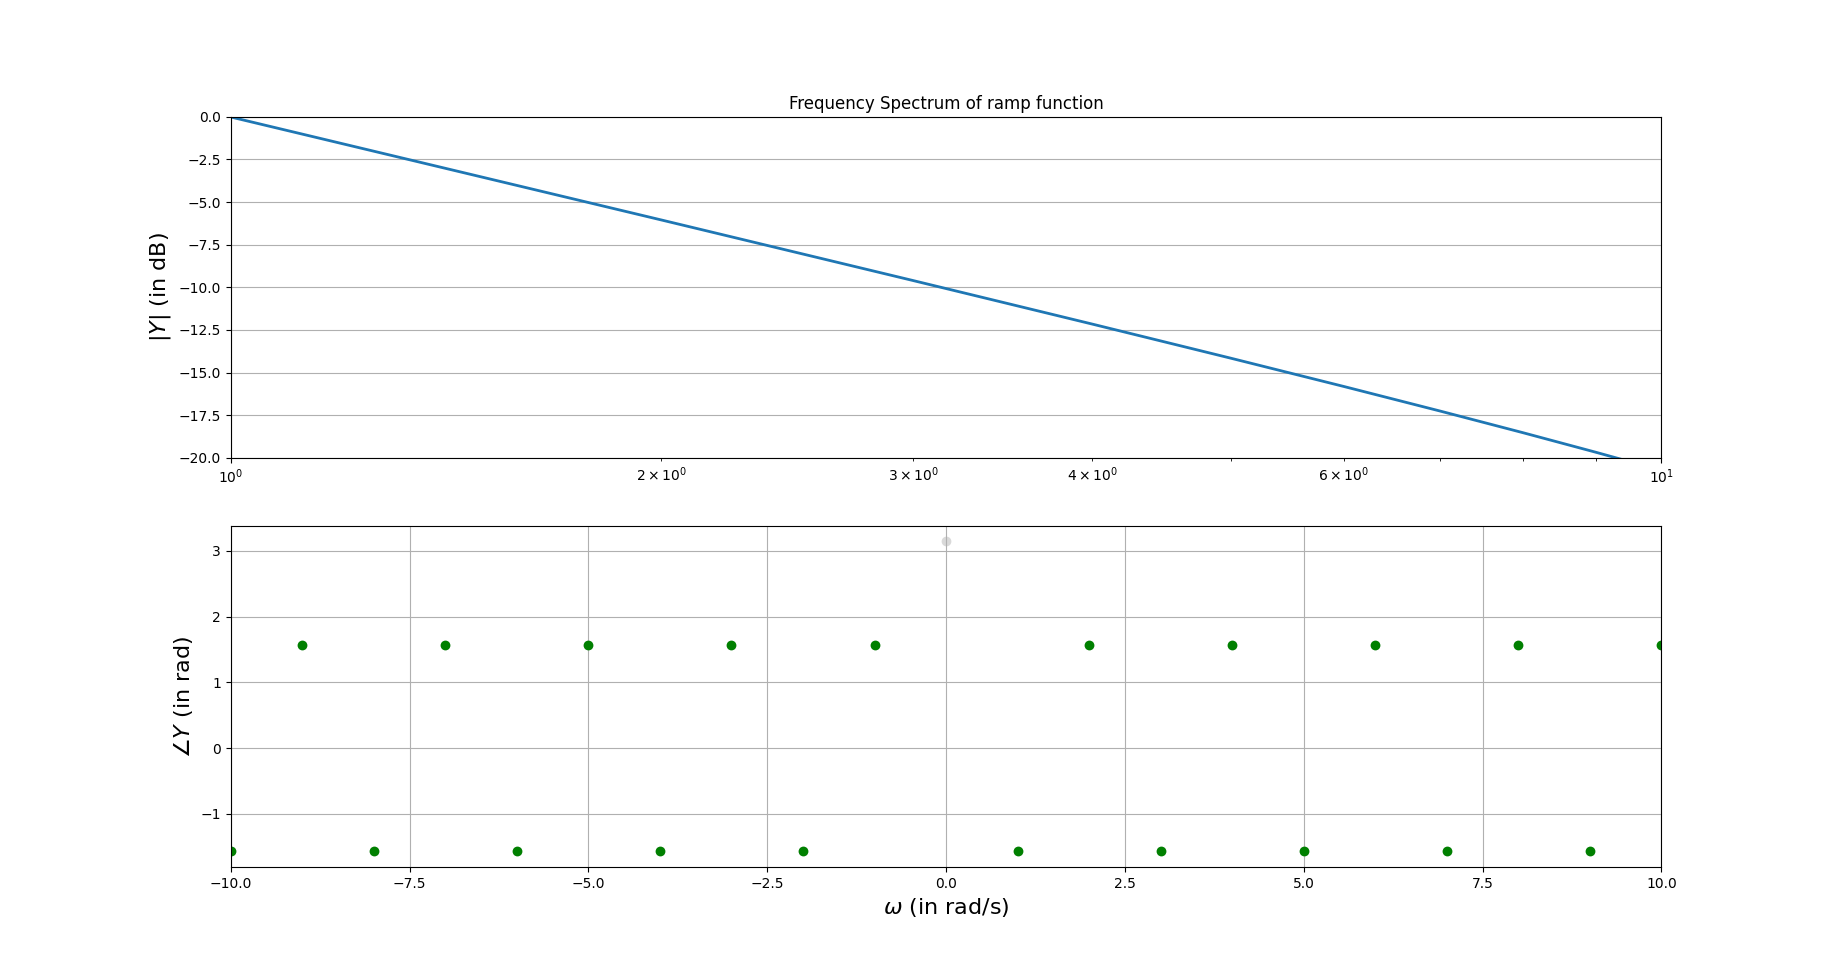
\includegraphics[scale=0.3]{Figure_1_3}}{\large\par}
\par\end{centering}
{\large{}\caption{{\large{}Frequency Spectrum of ramp function}}
}{\large\par}

\end{figure}
{\large\par}
\noindent \begin{flushleft}
{\large{}From the plot, we can say that the spectrum decays at the
rate of 20dB per decade (which is due to $1/\omega$). The big jump
at $n\pi$ force this slowly decaying spectrum, which is why we don't
see the expected spikes for the spectrum of $sin(\sqrt{2}t)$.}{\large\par}
\par\end{flushleft}

\subsection{Windowing:}
\noindent \begin{flushleft}
{\large{}Windowing is a technique to reduce the discontinuities by
damping the function near the discontinuities. For this we shall multiply
the given function sequency by a ``window'' sequence $w[n]$:}{\large\par}
\par\end{flushleft}

\begin{center}
{\large{}$g(n)=f(n)w(n)$}{\large\par}
\par\end{center}

\noindent \begin{flushleft}
{\large{}The Hamming Window function we will be using is the following:}{\large\par}
\par\end{flushleft}

\begin{center}
{\large{}$w[n]=\begin{cases}
0.54+0.46cos(\frac{2\pi n}{N-1}) & |n|\leq\frac{N-1}{2}\\
0 & else
\end{cases}$}{\large\par}
\par\end{center}

\noindent \begin{flushleft}
{\large{}Code snippet for windowing is as follows:}{\large\par}
\par\end{flushleft}

{\large{}}
\begin{lstlisting}[language=Python]
def HammingWindow(a, b, n):
    return fftshift(a + b * cos((2 * pi * n)/(len(n) - 1)))
\end{lstlisting}
{\large\par}
\noindent \begin{flushleft}
{\large{}Now let's plot the sinusoidal function after applying Hamming
Window.}{\large\par}
\par\end{flushleft}

{\large{}}
\begin{figure}[H]
\noindent \begin{centering}
{\large{}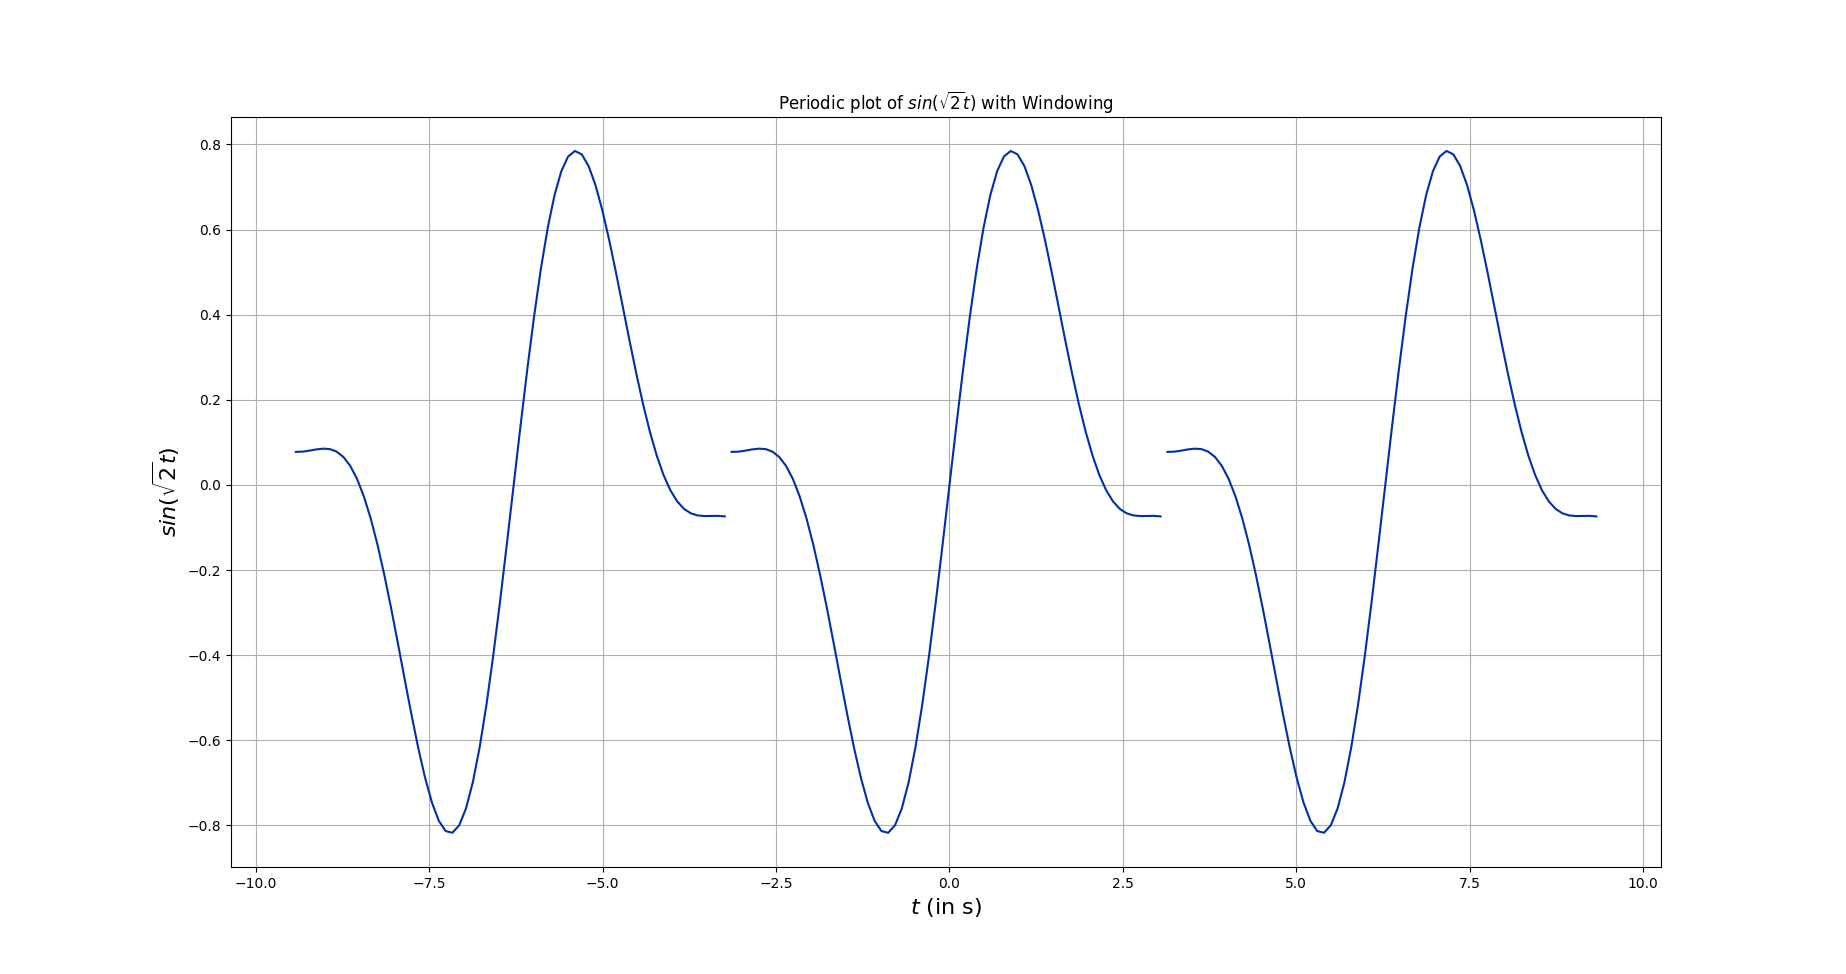
\includegraphics[scale=0.3]{Figure_1_4}}{\large\par}
\par\end{centering}
{\large{}\caption{{\large{}Periodic plot of $sin(\sqrt{2}t)$ after Windowing}}
}{\large\par}

\end{figure}
{\large\par}
\noindent \begin{flushleft}
{\large{}The discontinuity is reduced significantly. The corresponding
DFT plots are:}{\large\par}
\par\end{flushleft}

{\large{}}
\begin{figure}[H]
\begin{centering}
{\large{}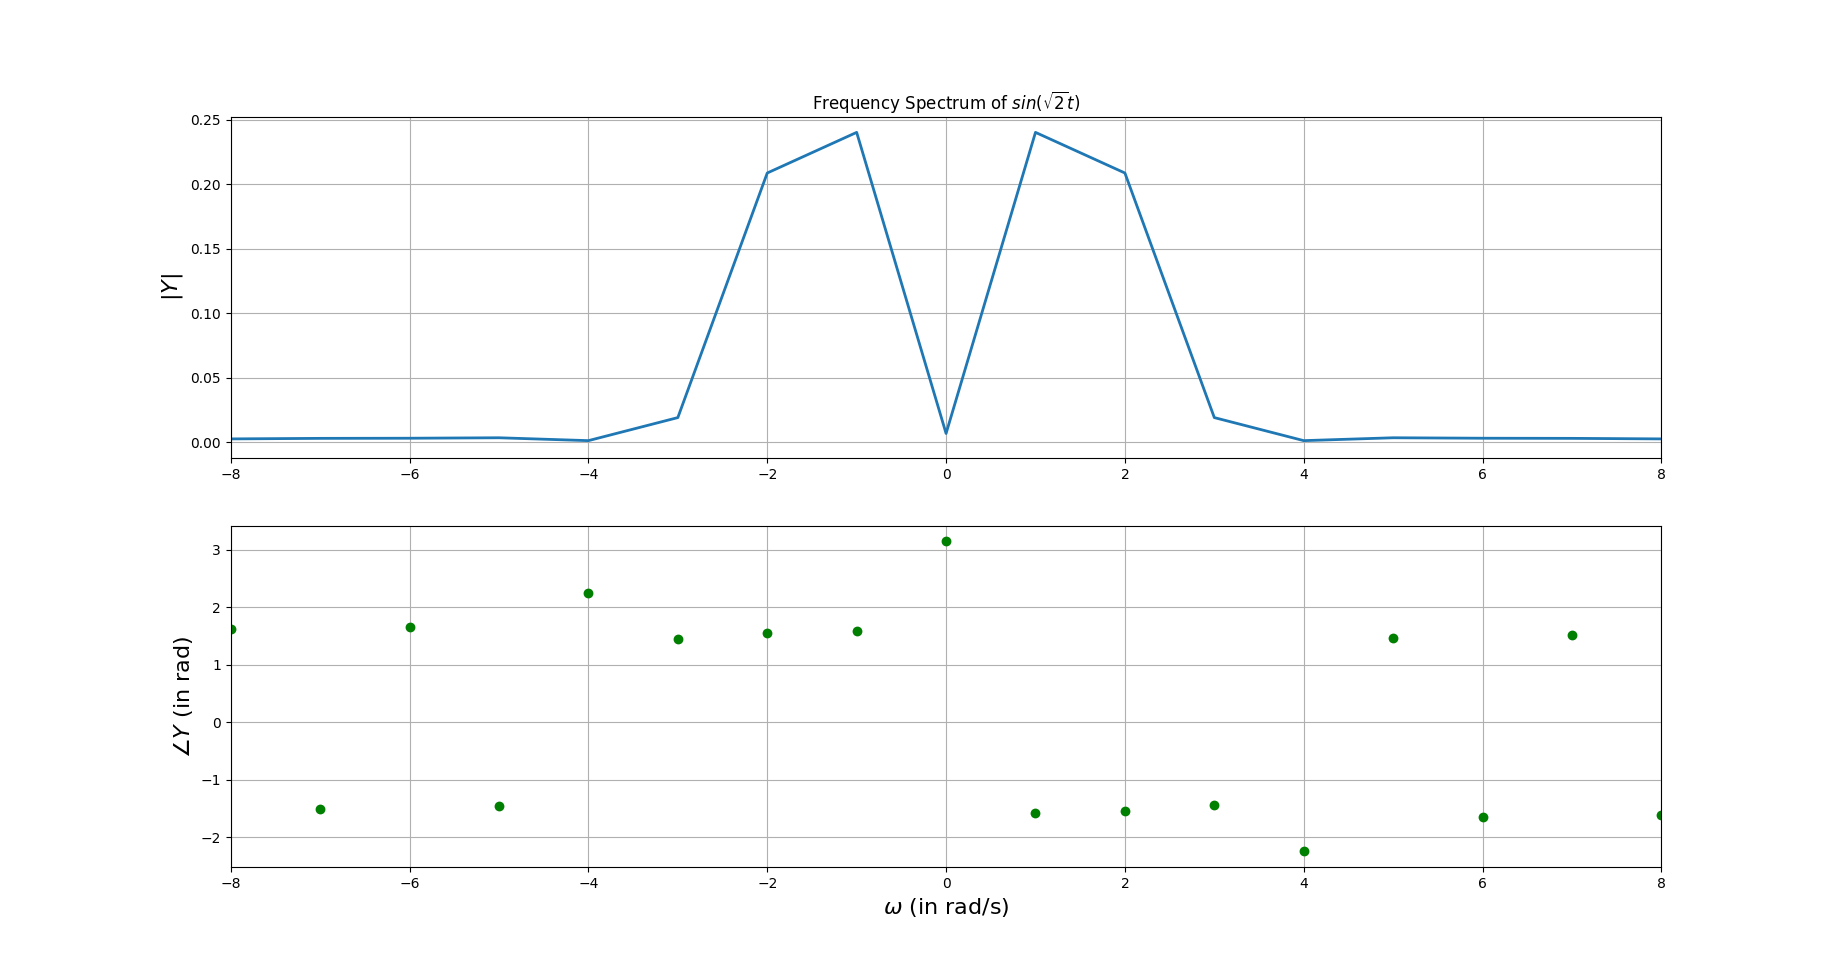
\includegraphics[scale=0.3]{Figure_1_5}}{\large\par}
\par\end{centering}
{\large{}\caption{{\large{}Frequency Spectrum of $sin(\sqrt{2}t)w(n)$}}
}{\large\par}

\end{figure}
{\large\par}
\noindent \begin{flushleft}
{\large{}The magnitude response is much better now as there is only
one peak. Let's try to increase the resolution to get better defined
peaks.}{\large\par}
\par\end{flushleft}

{\large{}}
\begin{figure}[H]
\begin{centering}
{\large{}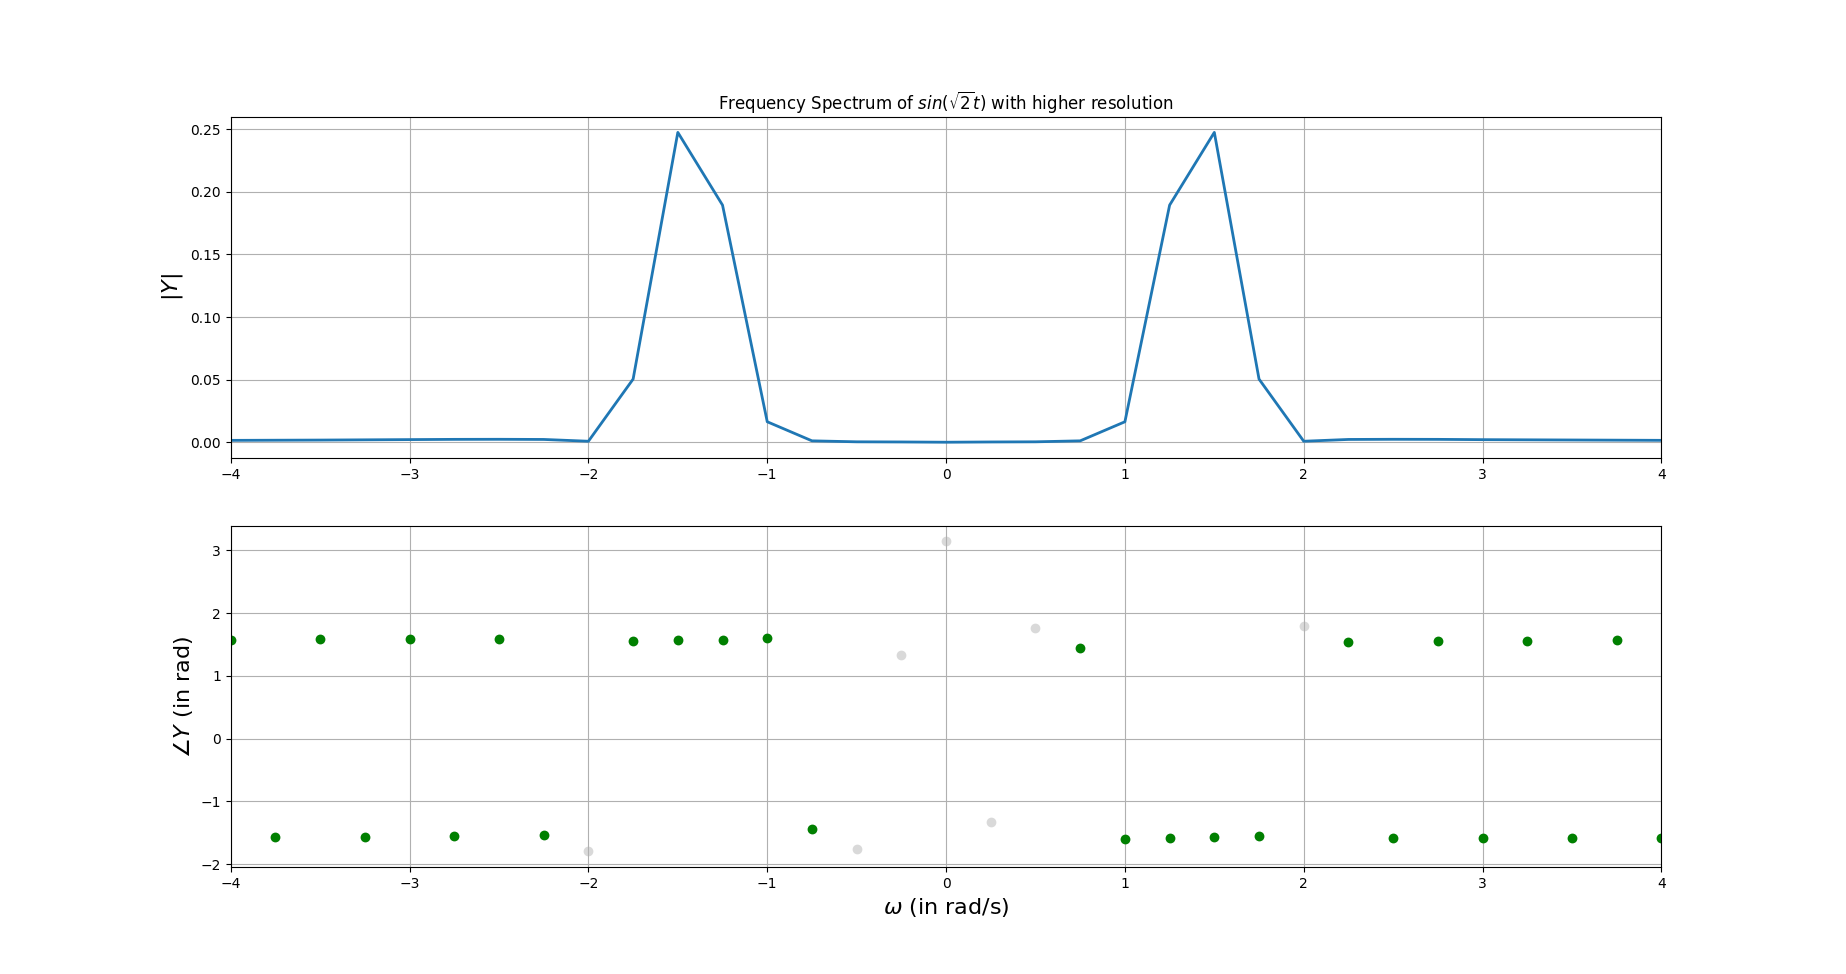
\includegraphics[scale=0.3]{Figure_1_6}}{\large\par}
\par\end{centering}
{\large{}\caption{{\large{}Frequency Spectrum of $sin(\sqrt{2}t)w(n)$ with higher resolution}}
}{\large\par}
\end{figure}
{\large\par}
\noindent \begin{flushleft}
{\large{}The peaks are more well defined and the magnitude response
falls more rapidly for higher values. We notice that the width of
the peaks have increased a bit with windowing. Let's test this with
another sinusoid.}{\large\par}
\par\end{flushleft}

{\large{}}
\begin{figure}[H]
\begin{centering}
{\large{}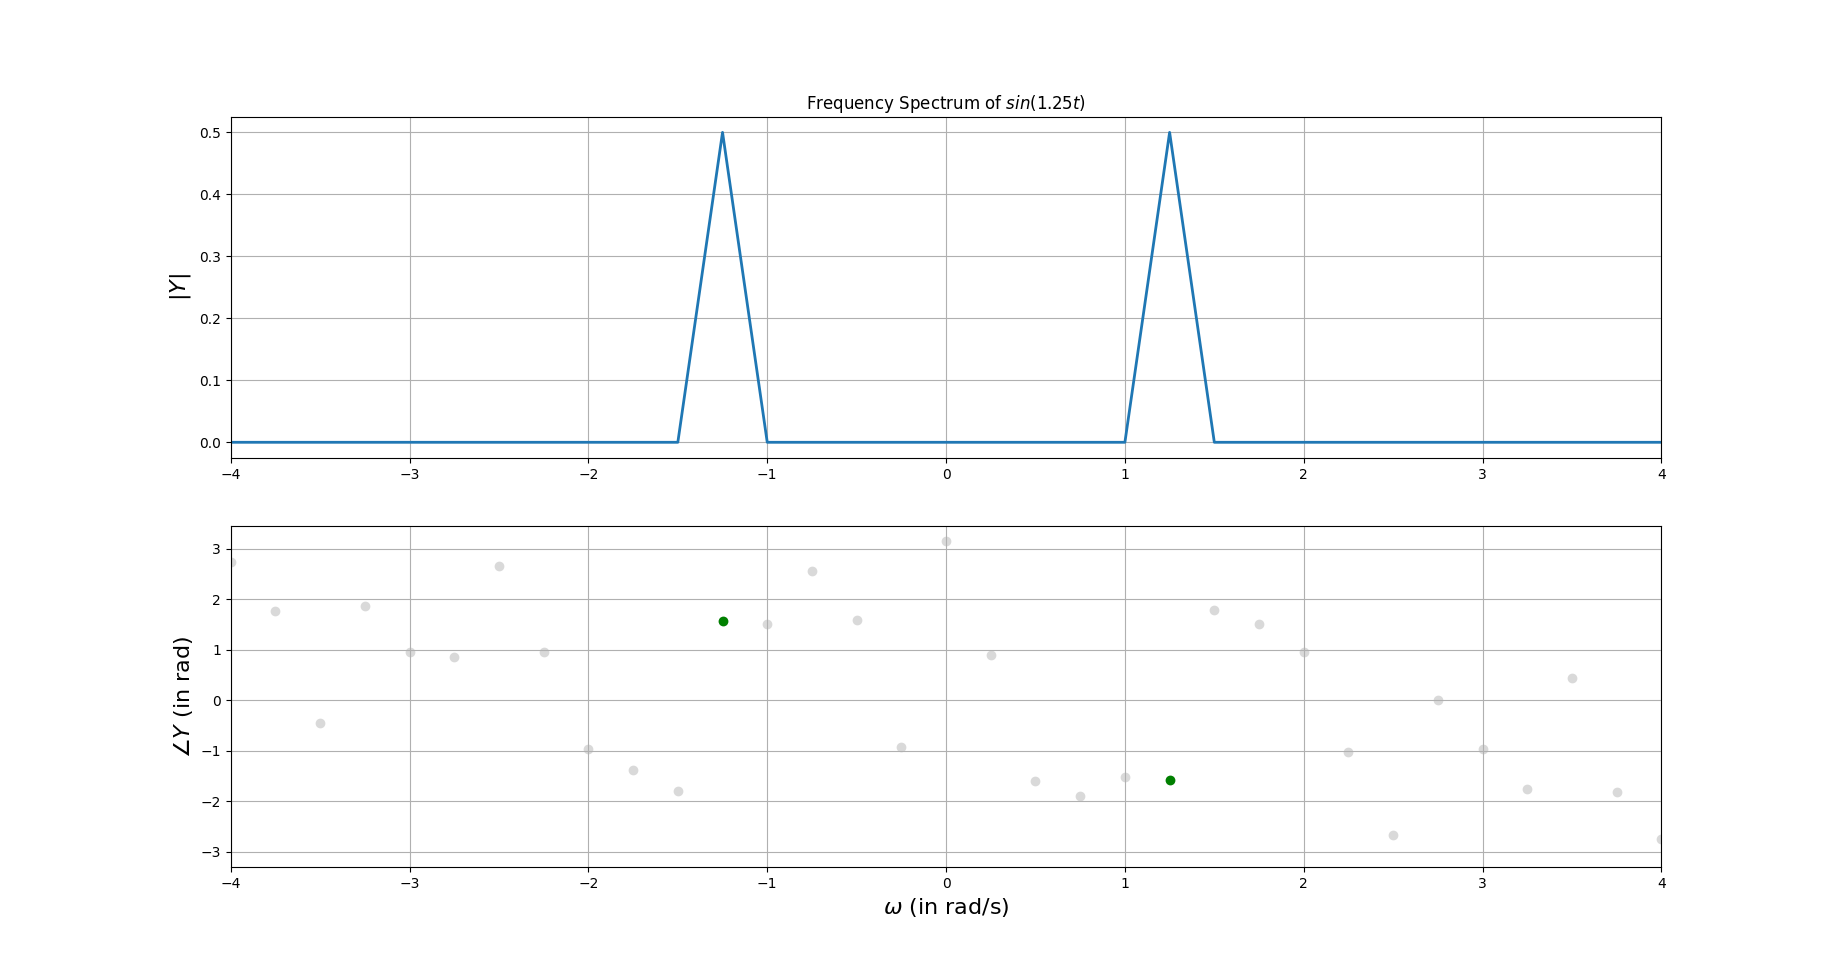
\includegraphics[scale=0.3]{Figure_1_7}}{\large\par}
\par\end{centering}
{\large{}\caption{{\large{}Frequency Spectrum of $sin(1.25t)$ without Windowing}}
}{\large\par}
\end{figure}
{\large\par}

{\large{}}
\begin{figure}[H]
\noindent \begin{centering}
{\large{}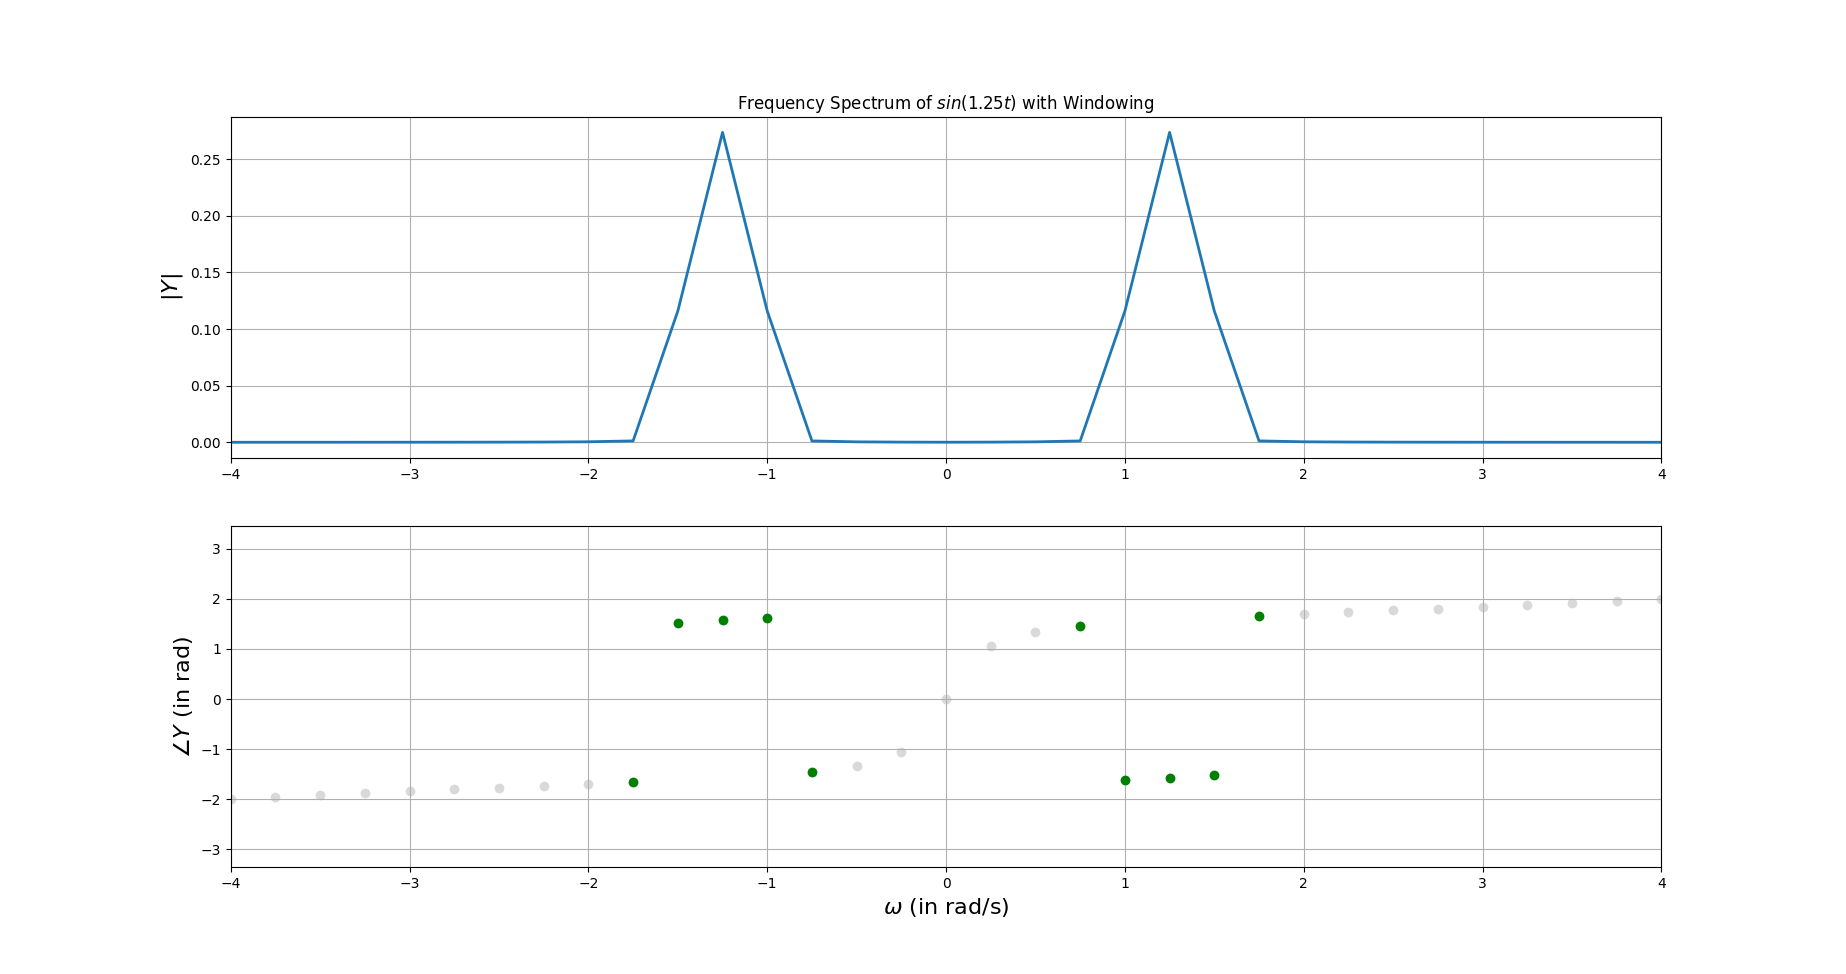
\includegraphics[scale=0.3]{Figure_1_8}}{\large\par}
\par\end{centering}
{\large{}\caption{{\large{}Frequency Spectrum of $sin(1.25t)$ with Windowing}}
}{\large\par}
\end{figure}
{\large\par}

\noindent {\large{}For the same resolution, Hamming Window is actually
increasing the width of the peak. This would create a problem if our
resolution is not sufficiently high.}{\large\par}

\subsection{DFT Analysis of $cos^{3}(\omega_{0}t)$:}
\noindent \begin{flushleft}
{\large{}Let's follow the same procedure for $cos^{3}(\omega_{0}t)$
with $\omega_{0}=0.86$.}{\large\par}
\par\end{flushleft}

\begin{center}
{\large{}$cos^{3}(0.86t)=\frac{1}{4}cos(3(0.86)t)+\frac{3}{4}cos(0.86t)$ }{\large\par}
\par\end{center}

\noindent \begin{flushleft}
{\large{}So we expect the peaks to be at $\pm0.86$ and $\pm2.58$.}{\large\par}
\par\end{flushleft}

{\large{}}
\begin{figure}[H]
\begin{centering}
{\large{}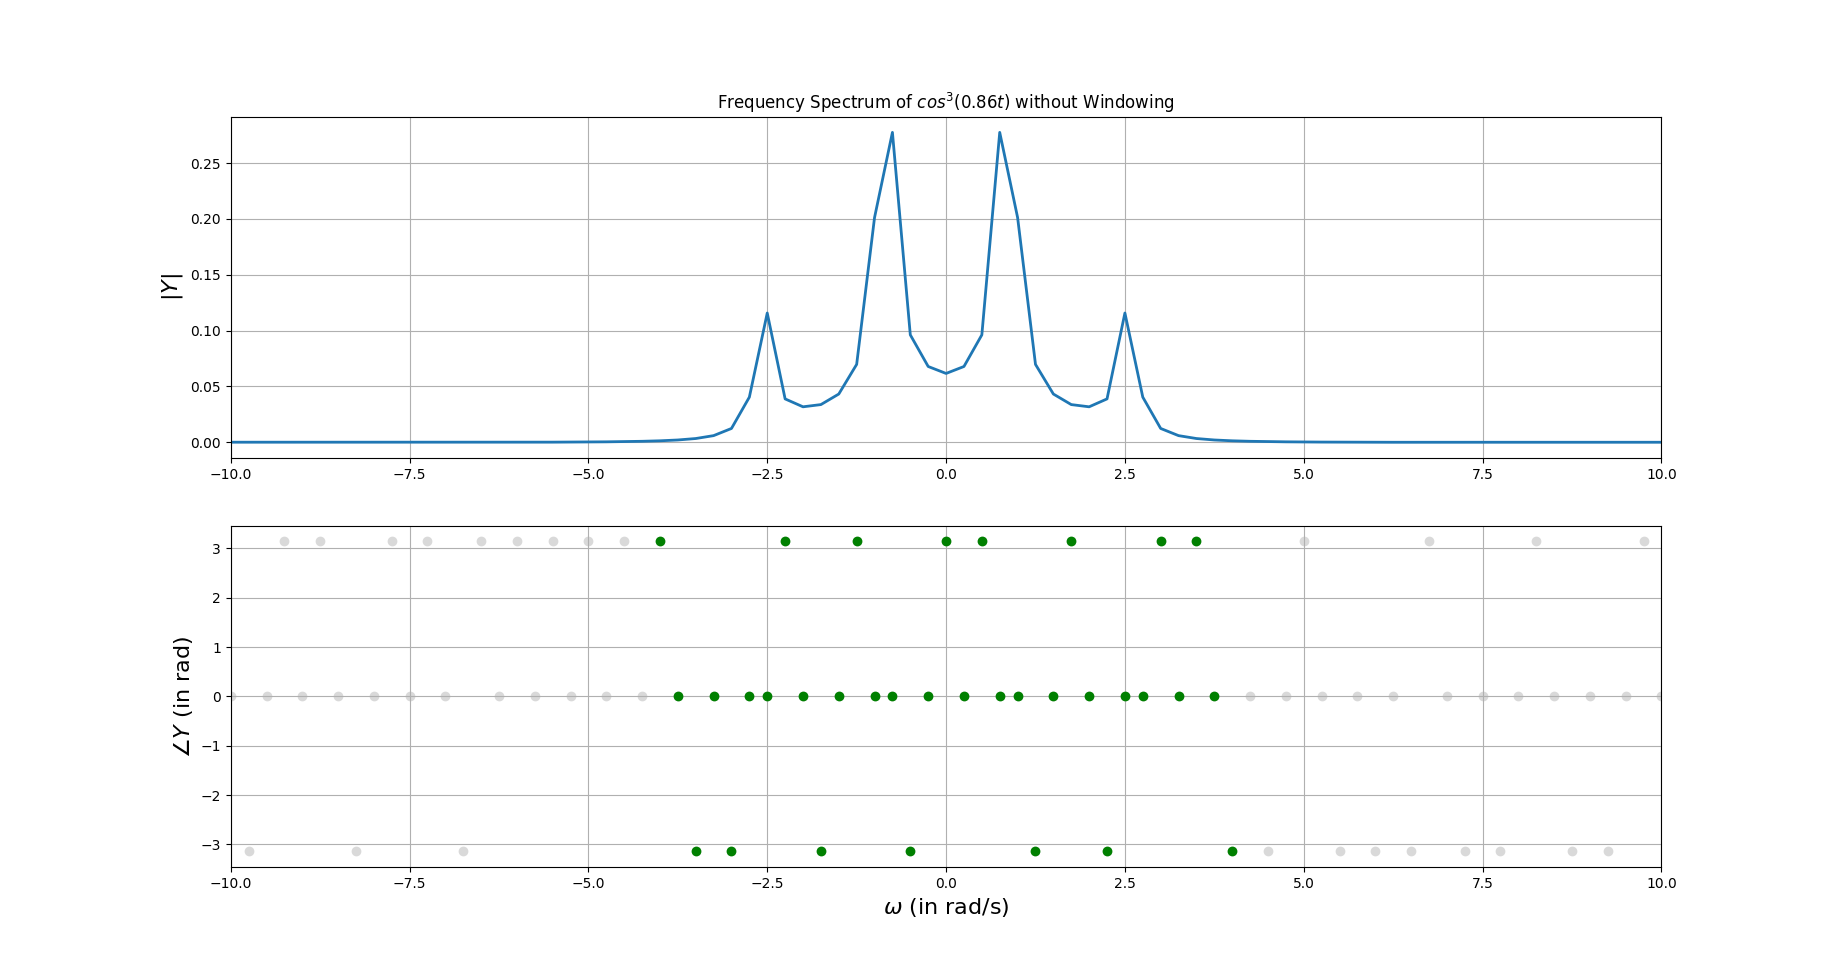
\includegraphics[scale=0.3]{Figure_2}}{\large\par}
\par\end{centering}
{\large{}\caption{{\large{}Frequency Spectrum of $cos^{3}(0.86t)$ without Windowing}}
}{\large\par}

\end{figure}
{\large\par}

{\large{}}
\begin{figure}[H]
\begin{centering}
{\large{}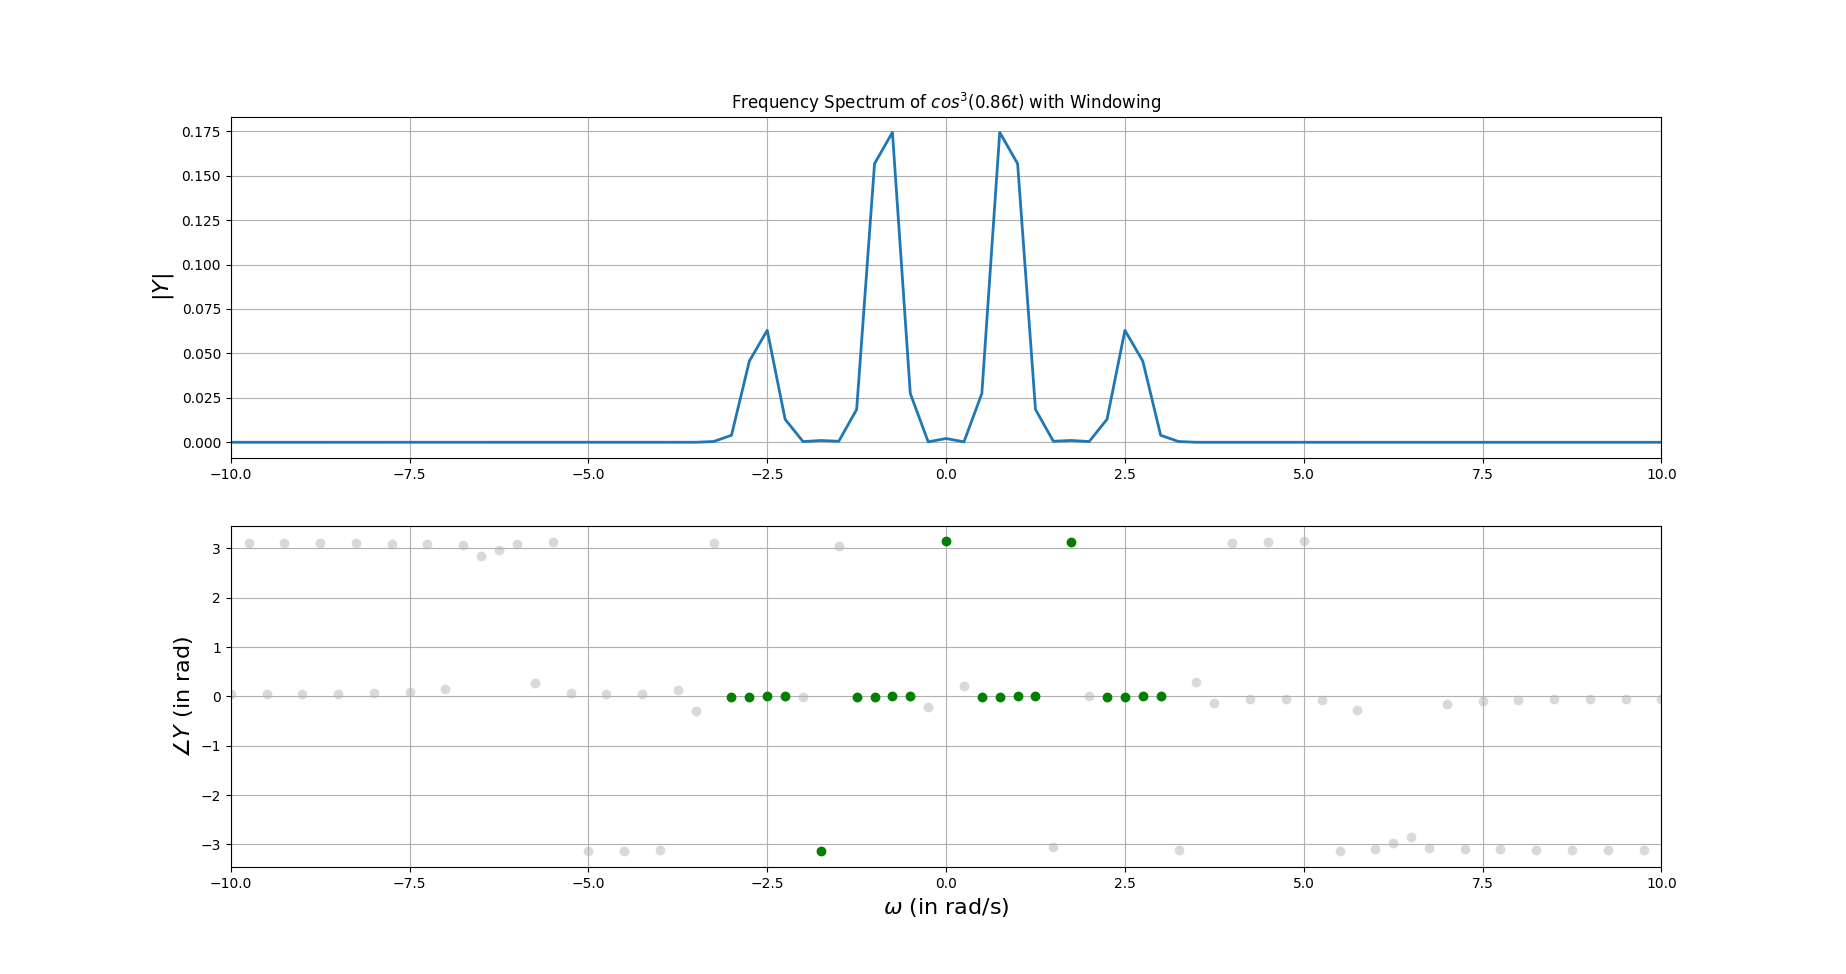
\includegraphics[scale=0.3]{Figure_2_2}}{\large\par}
\par\end{centering}
{\large{}\caption{{\large{}Frequency Spectrum of $cos^{3}(0.86t)$ with Windowing}}
}{\large\par}

\end{figure}
{\large\par}
\noindent \begin{flushleft}
{\large{}We get the plots as expected with and without the Hamming
Window.}{\large\par}
\par\end{flushleft}

\subsection{DFT Analysis of $cos(\omega_{0}t+\delta)$:}
\noindent \begin{flushleft}
{\large{}Let's follow the same procedure for $cos(\omega_{0}t+\delta)$
with $\omega_{0}=0.6$ and $\delta=1$. We would expect the peaks
of the frequency spectrum to be located at $\pm\omega_{0}$.}{\large\par}
\par\end{flushleft}

{\large{}}
\begin{figure}[H]
\begin{centering}
{\large{}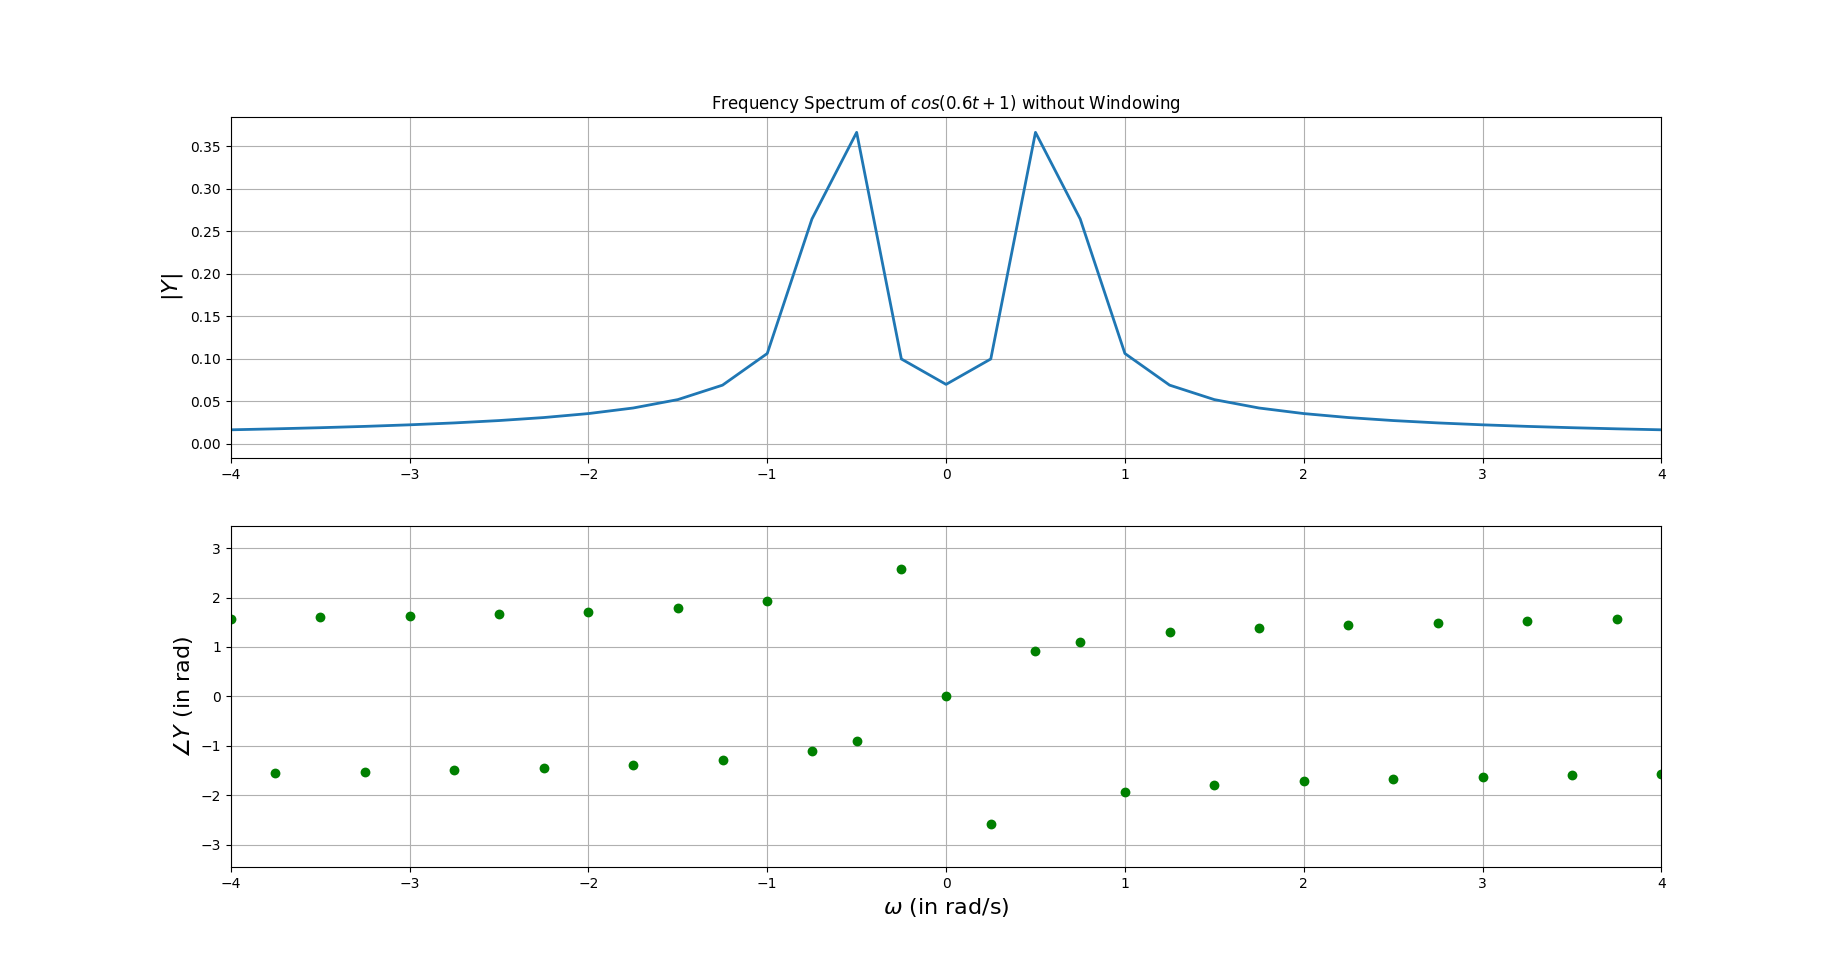
\includegraphics[scale=0.3]{Figure_3}}{\large\par}
\par\end{centering}
{\large{}\caption{{\large{}Frequency Spectrum of $cos(0.6t+1)$ without Windowing}}
}{\large\par}

\end{figure}
{\large\par}

{\large{}}
\begin{figure}[H]
\begin{centering}
{\large{}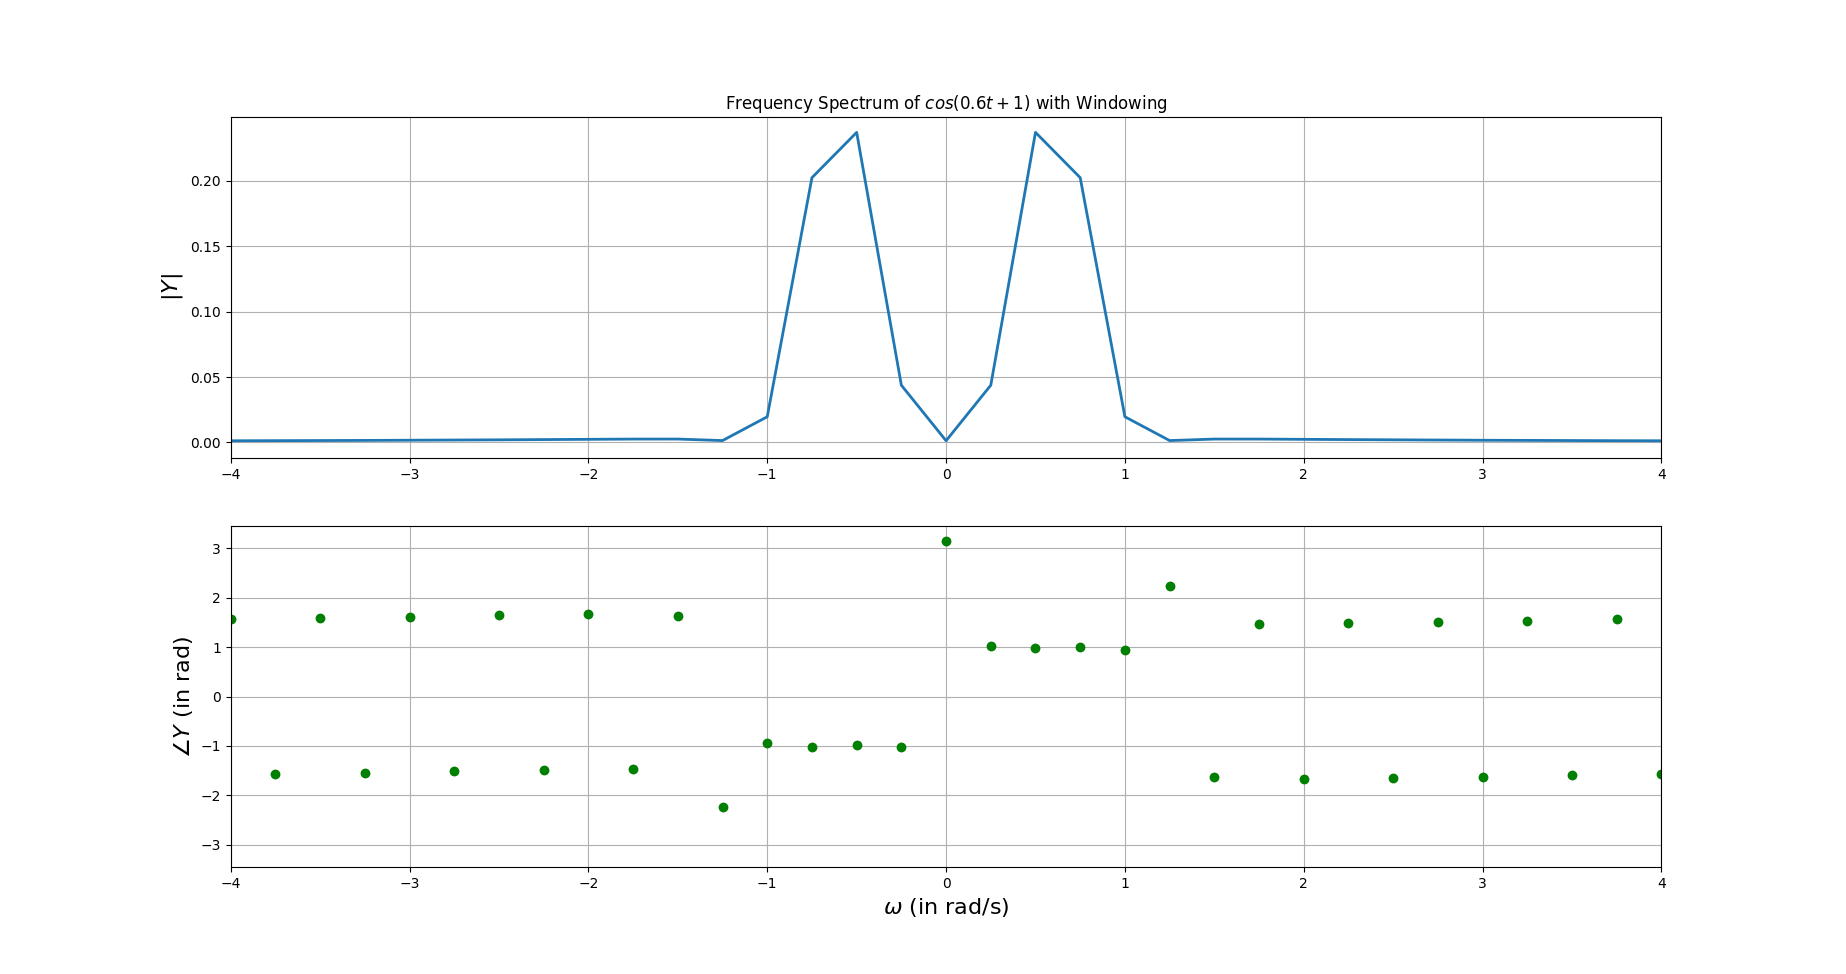
\includegraphics[scale=0.3]{Figure_3_2}}{\large\par}
\par\end{centering}
{\large{}\caption{{\large{}Frequency Spectrum of $cos(0.6t+1)$ with Windowing}}
}{\large\par}

\end{figure}
{\large\par}
\noindent \begin{flushleft}
{\large{}From the plots, we can see that the peaks are approximately
at $\pm0.6$.}{\large\par}
\par\end{flushleft}

\noindent \begin{flushleft}
{\large{}We can also try to estimate more accurately the values by
performing a weighted average with the magnitude squared being the
weight for all the frequencies under the peak. The code snippet for
estimating $\omega_{0}$ and $\delta$ is as follows:}{\large\par}
\par\end{flushleft}

\begin{lstlisting}[language=Python]
def estimate(w, mag, phase):
    actual_mag = where(mag > 0.2)

    w_avg = sum((mag[actual_mag]**2) * abs(w[actual_mag]))/sum(mag[actual_mag]**2)

    phase_avg = mean(abs(phase[actual_mag]))

    print("Estimated w0:", w_avg)
    print("Estimated delta:", phase_avg)
\end{lstlisting}

\begin{lstlisting}
Estimations for cos(0.6t+1):
Estimated w0: 0.5856280489361705
Estimated delta: 1.0062163015426053

Estimations for cos(0.6t+1)w(t):
Estimated w0: 0.6054218881468985
Estimated delta: 1.0010884777925986
\end{lstlisting}

\noindent \begin{flushleft}
{\large{}The estimated values are very close to actual values.}{\large\par}
\par\end{flushleft}

\subsection{DFT Analysis of $cos(\omega_{0}t+\delta)$ with added white gaussian
noise:}
\noindent \begin{flushleft}
{\large{}We shall now add some white gaussian noise to the previous
cosine signal. So the resulting signal will be:}{\large\par}
\par\end{flushleft}

{\large{}}
\begin{lstlisting}[language=Python]
def cos_delta_with_noise(x):
    return cos(0.6 * x + 1) + 0.1 * randn(len(x))
\end{lstlisting}
{\large\par}
\noindent \begin{flushleft}
{\large{}We shall perform the same analysis for this too:}{\large\par}
\par\end{flushleft}

{\large{}}
\begin{figure}[H]
\begin{centering}
{\large{}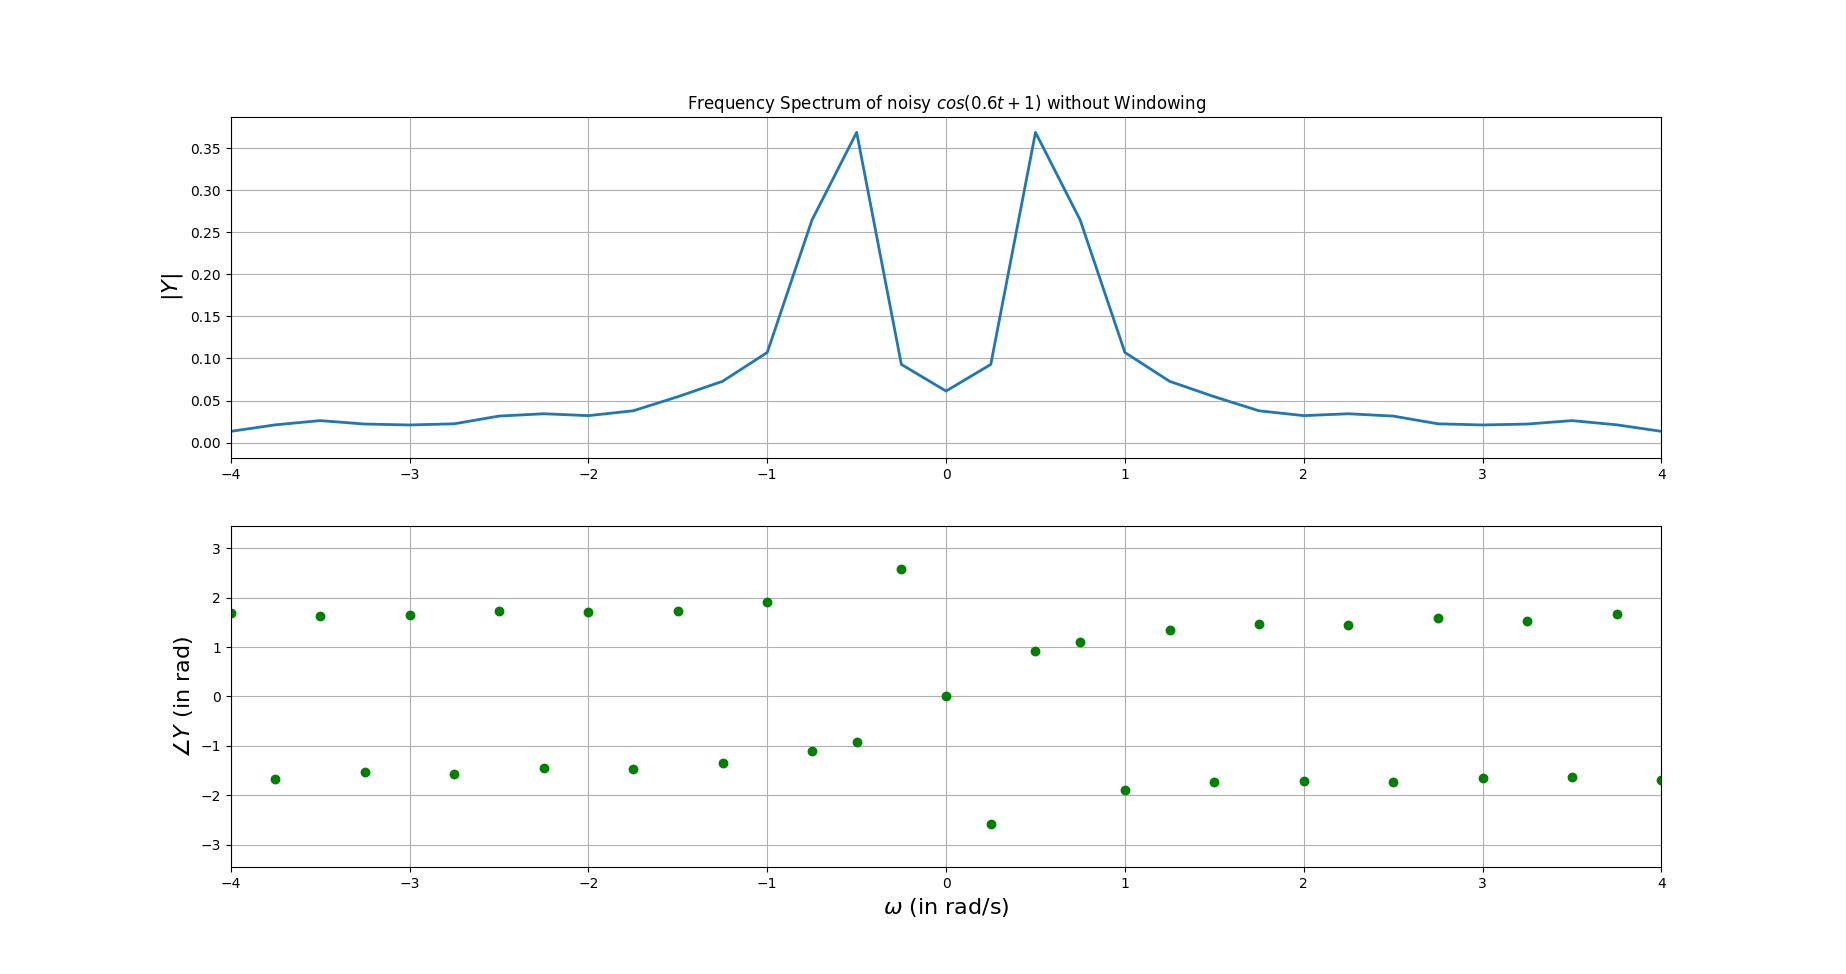
\includegraphics[scale=0.3]{Figure_4}}{\large\par}
\par\end{centering}
{\large{}\caption{{\large{}Frequency Spectrum of noisy $cos(0.6t+1)$ without Windowing}}
}{\large\par}
\end{figure}
{\large\par}

{\large{}}
\begin{figure}[H]
\begin{centering}
{\large{}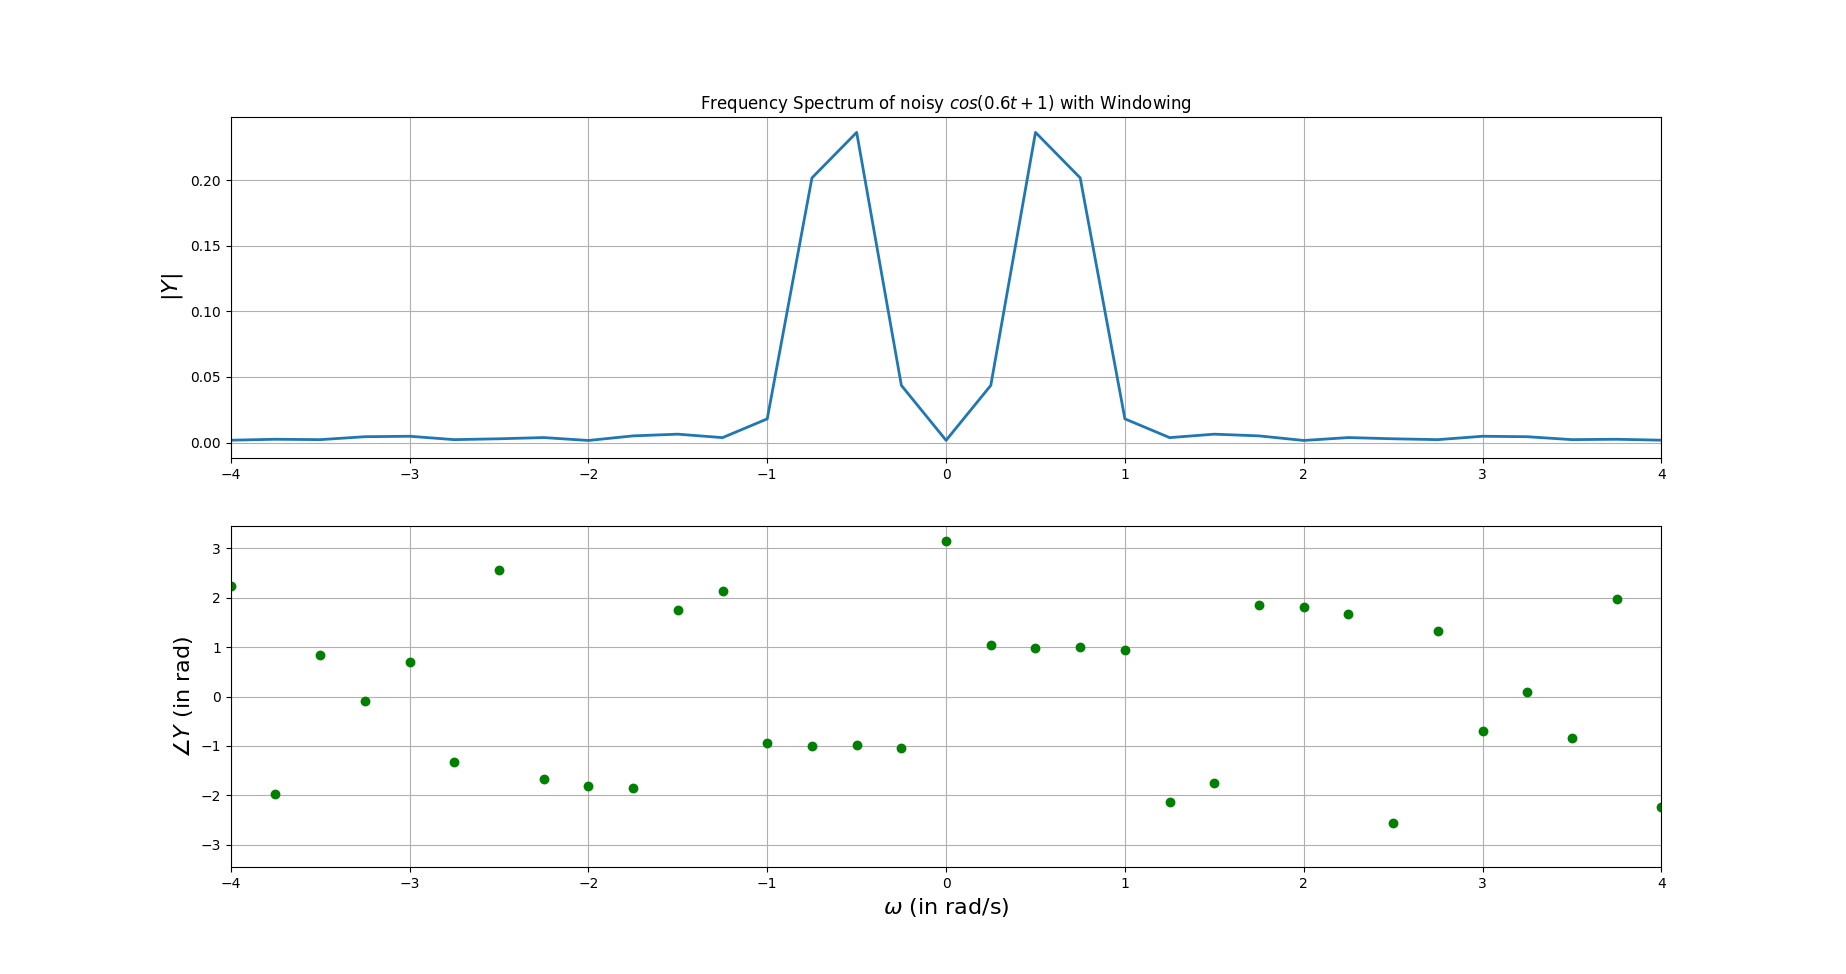
\includegraphics[scale=0.3]{Figure_4_2}}{\large\par}
\par\end{centering}
{\large{}\caption{{\large{}Frequency Spectrum of noisy $cos(0.6t+1)$ with Windowing}}
}{\large\par}

\end{figure}
{\large\par}
\noindent \begin{flushleft}
{\large{}As we can see, there is a very small distortion in the frequency
spectra. We can also do the same estimation of $\omega_{0}$ and $\delta$.}{\large\par}
\par\end{flushleft}

\begin{lstlisting}
Estimations for noisy cos(0.6t+1):
Estimated w0: 0.5849385977821686
Estimated delta: 0.999694716712083

Estimations for noisy cos(0.6t+1)w(t):
Estimated w0: 0.6043866653600212
Estimated delta: 1.0027201730163195
\end{lstlisting}

\noindent \begin{flushleft}
{\large{}As we can see, the values estimated are very close to the
actual values. There is very less effect due to the noise. Let us
look at the effect for higher noise:}{\large\par}
\par\end{flushleft}

\begin{lstlisting}
Estimations for noisy cos(0.6t+1):
Estimated w0: 0.5872547551846261
Estimated delta: 1.05992394655917

Estimations for noisy cos(0.6t+1)w(t):
Estimated w0: 0.6184164246038958
Estimated delta: 1.0089962410560627
\end{lstlisting}

\noindent {\large{}For 10 times more noise, the error increased very
slightly.}{\large\par}

\subsection{DFT Analysis of Chirped signal:}
\begin{flushleft}
{\large{}Let's first have a look at the plots for a chirped signal
which is given by:}{\large\par}
\par\end{flushleft}

\begin{center}
{\large{}$f(t)=cos(16(1.5+\frac{t}{2\pi})t)$ }{\large\par}
\par\end{center}

{\large{}}
\begin{figure}[H]
\begin{centering}
{\large{}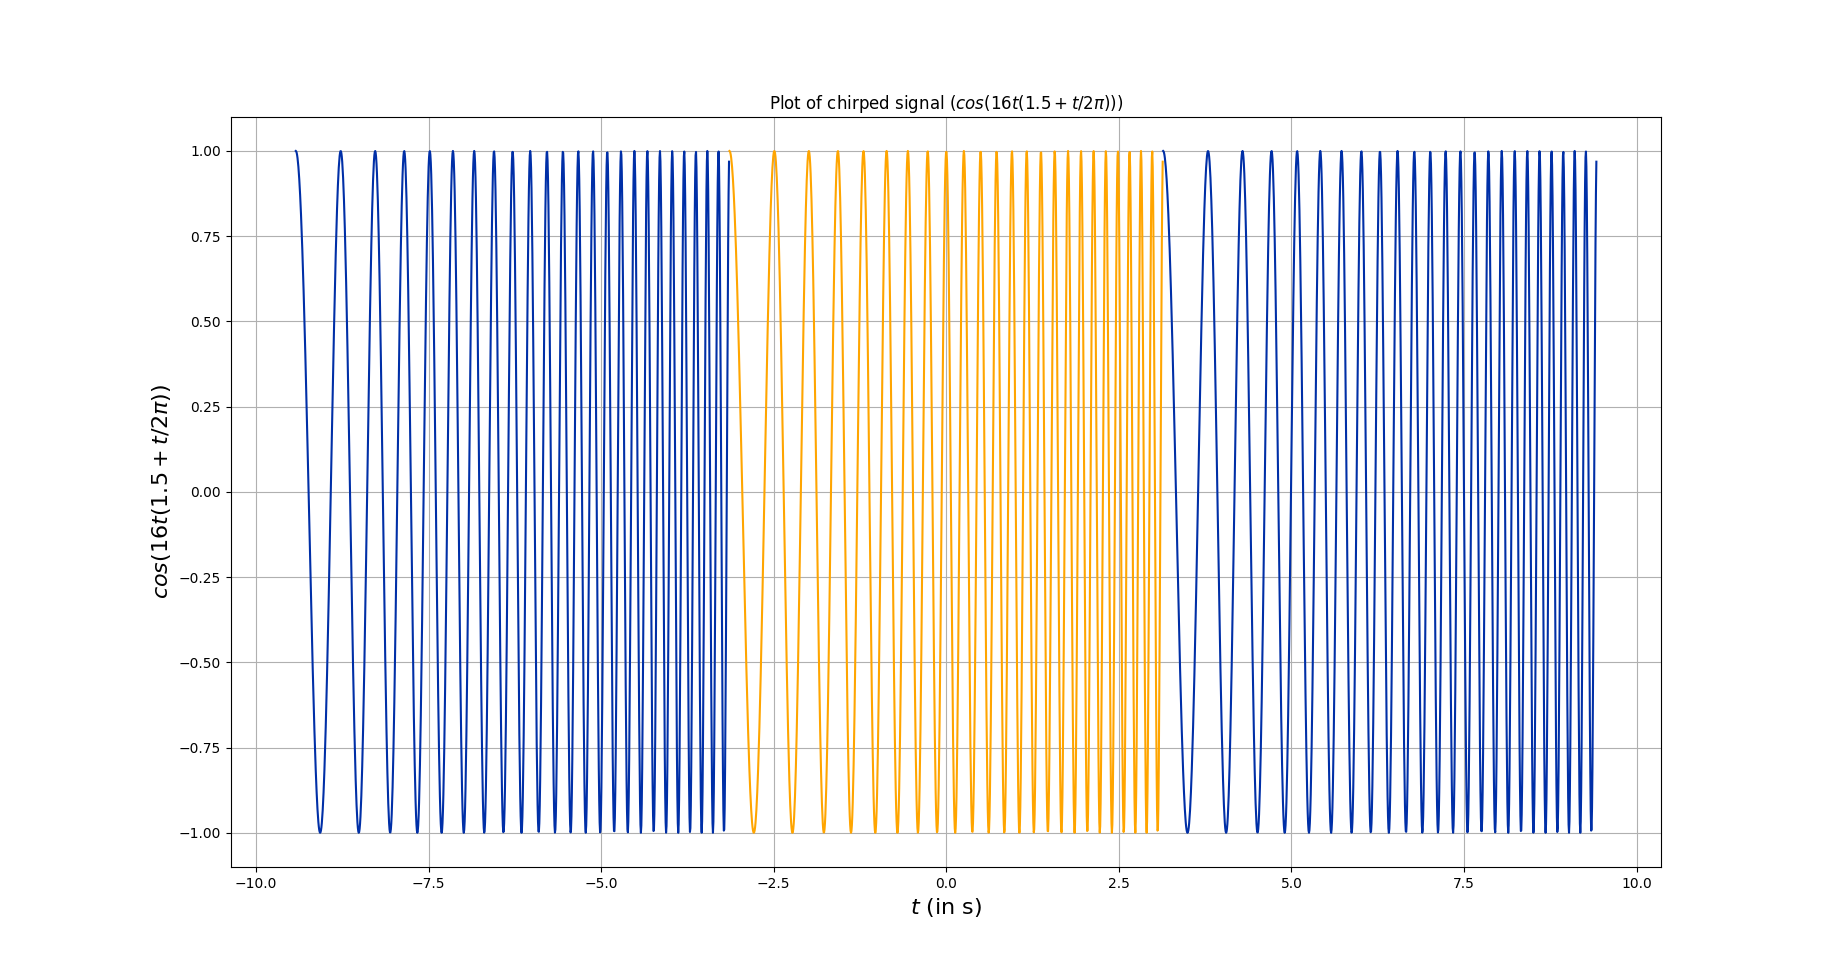
\includegraphics[scale=0.3]{chirp1}}{\large\par}
\par\end{centering}
{\large{}\caption{{\large{}Periodic approximation of chirped signal}}
}{\large\par}
\end{figure}
{\large\par}

{\large{}}
\begin{figure}[H]
\begin{centering}
{\large{}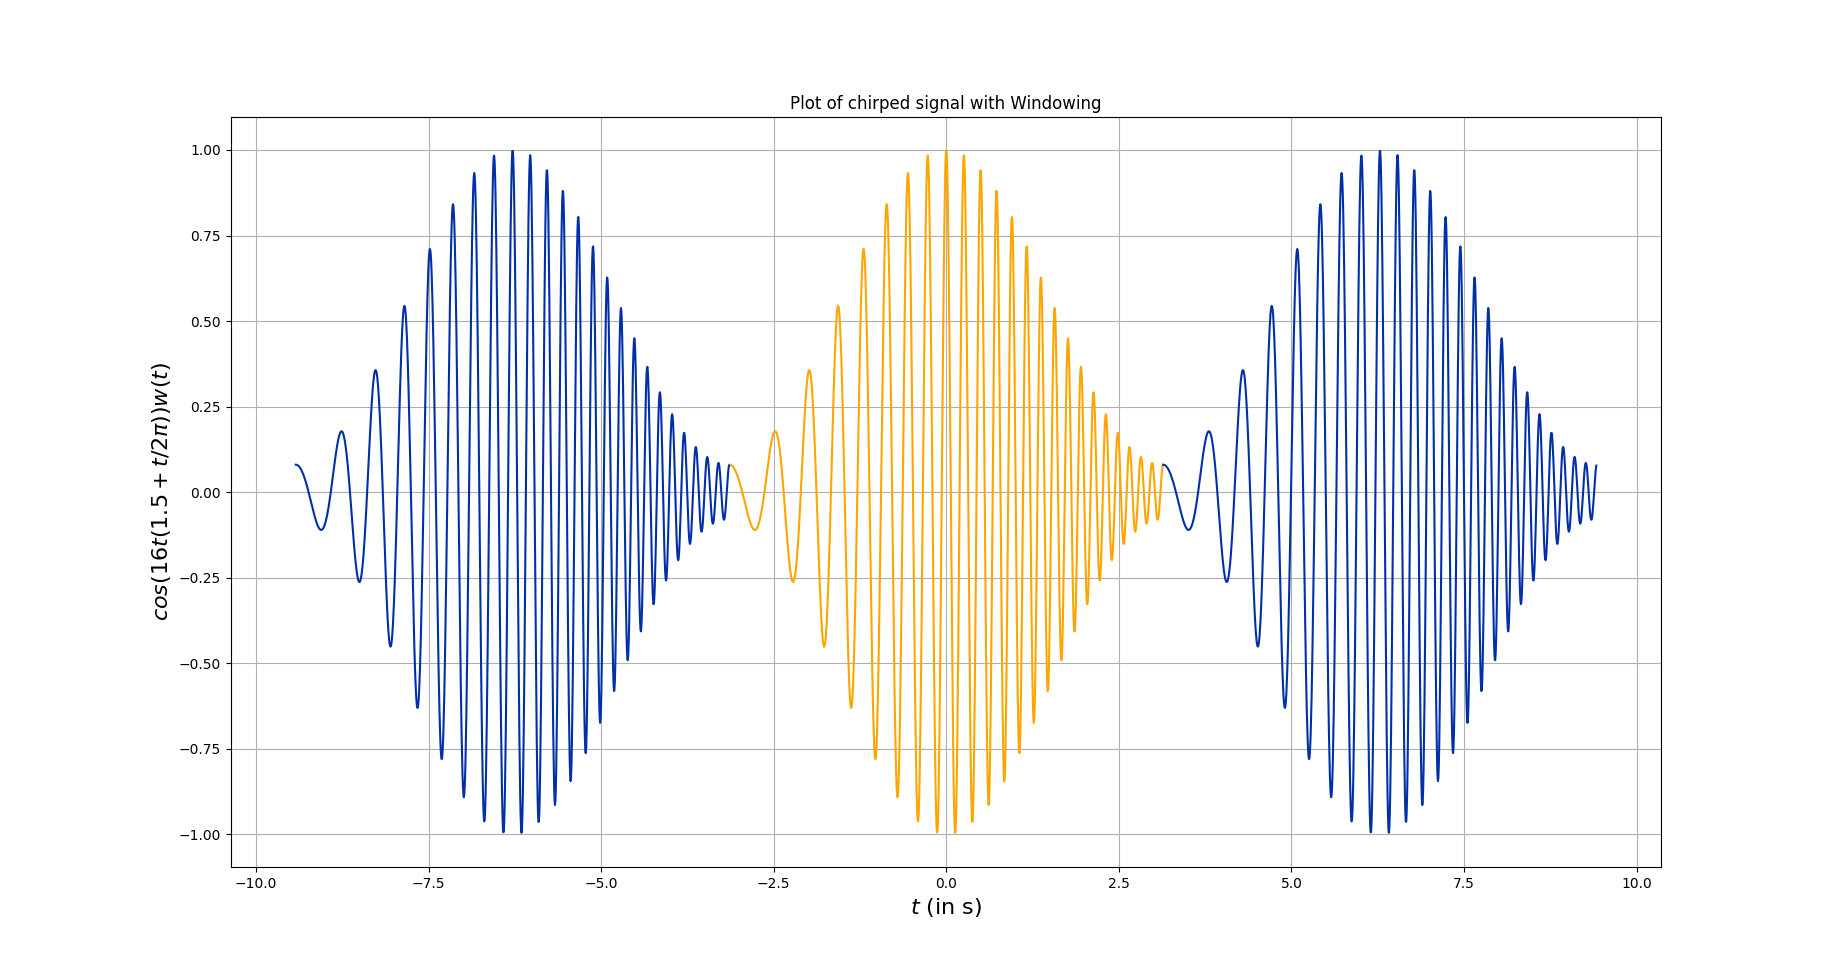
\includegraphics[scale=0.3]{chirp2}}{\large\par}
\par\end{centering}
{\large{}\caption{{\large{}Chirp signal with Windowing}}
}{\large\par}

\end{figure}
{\large\par}
\noindent \begin{flushleft}
{\large{}As we can see, the discontinuity appears to have been made
neglible by windowing. Code snippet for chirped signal:}{\large\par}
\par\end{flushleft}

{\large{}}
\begin{lstlisting}[language=Python]
## Function definition for chirp function
def chirp(x):
    return cos(16 * x * (1.5 + x/(2 * pi)))

## Function definition for chirp function with Windowing
def chirp_hamming(x):
    return chirp(x) * HammingWindow(0.54, 0.46, arange(len(x)))
\end{lstlisting}
{\large\par}

\pagebreak{}
\noindent \begin{flushleft}
{\large{}Plots of Magnitude and Phase response for a chirped signal:}{\large\par}
\par\end{flushleft}

{\large{}}
\begin{figure}[H]
\begin{centering}
{\large{}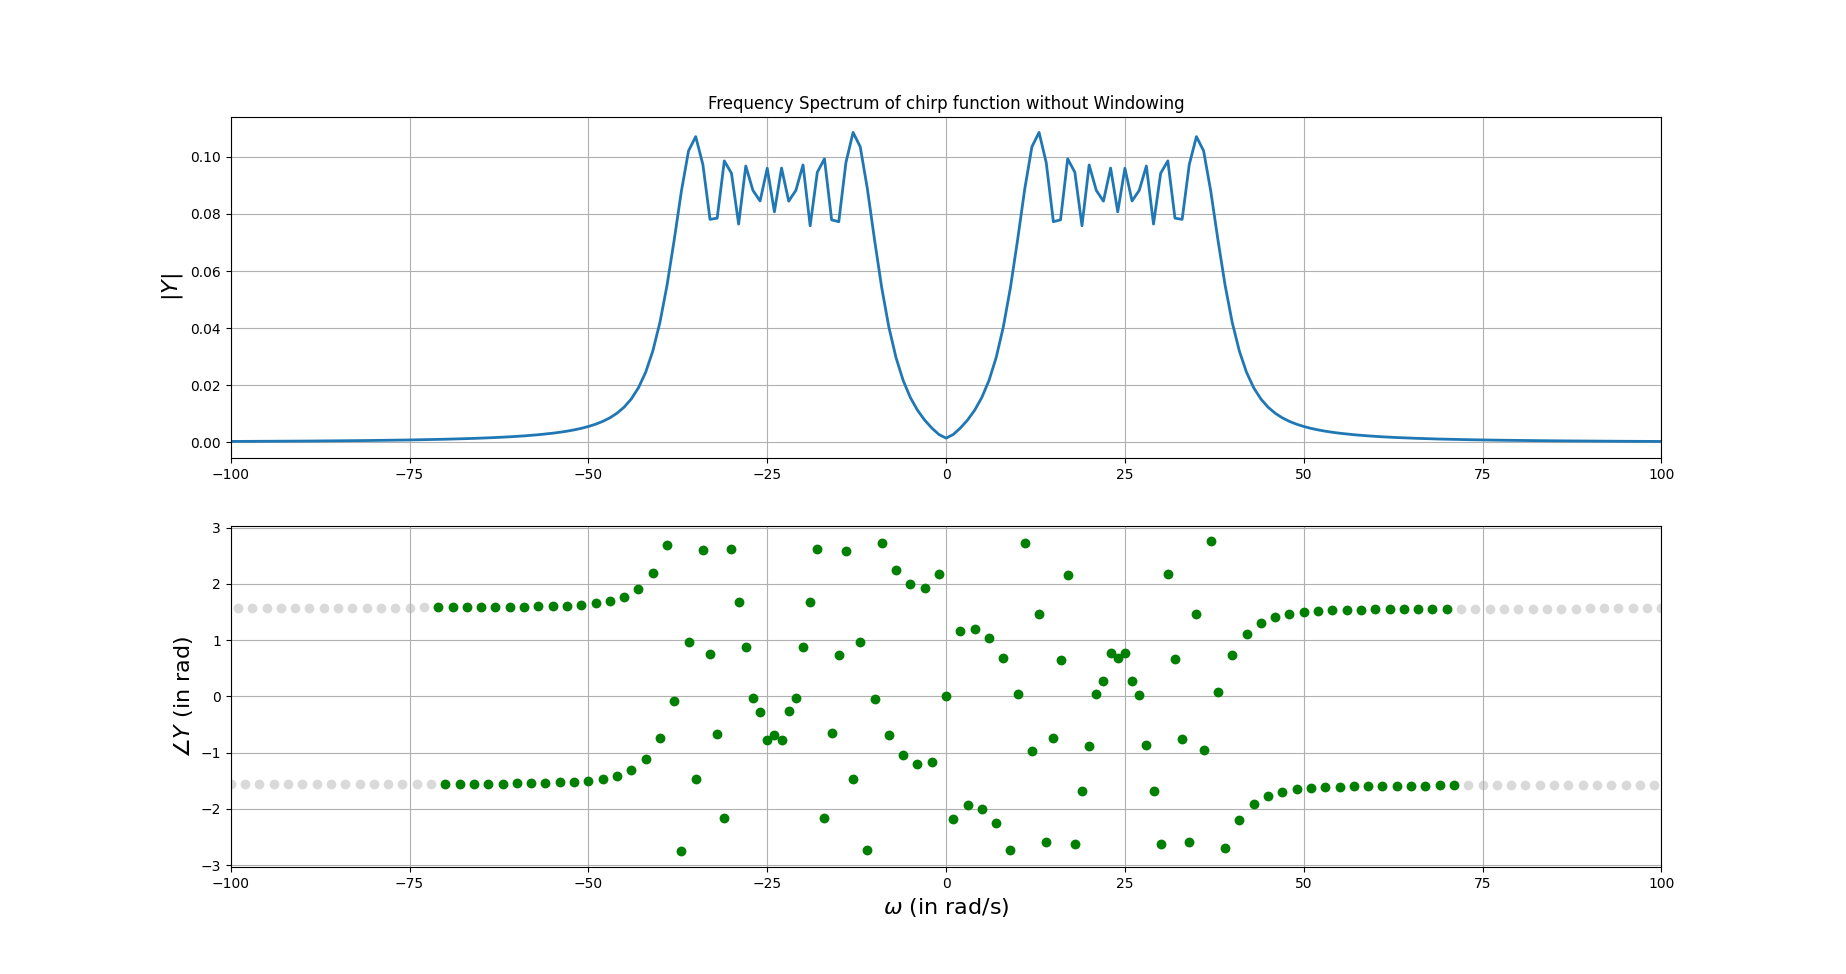
\includegraphics[scale=0.3]{Figure_5}}{\large\par}
\par\end{centering}
{\large{}\caption{{\large{}Frequency Spectrum of chirp function without Windowing}}
}{\large\par}
\end{figure}
{\large\par}

{\large{}}
\begin{figure}[H]
\begin{centering}
{\large{}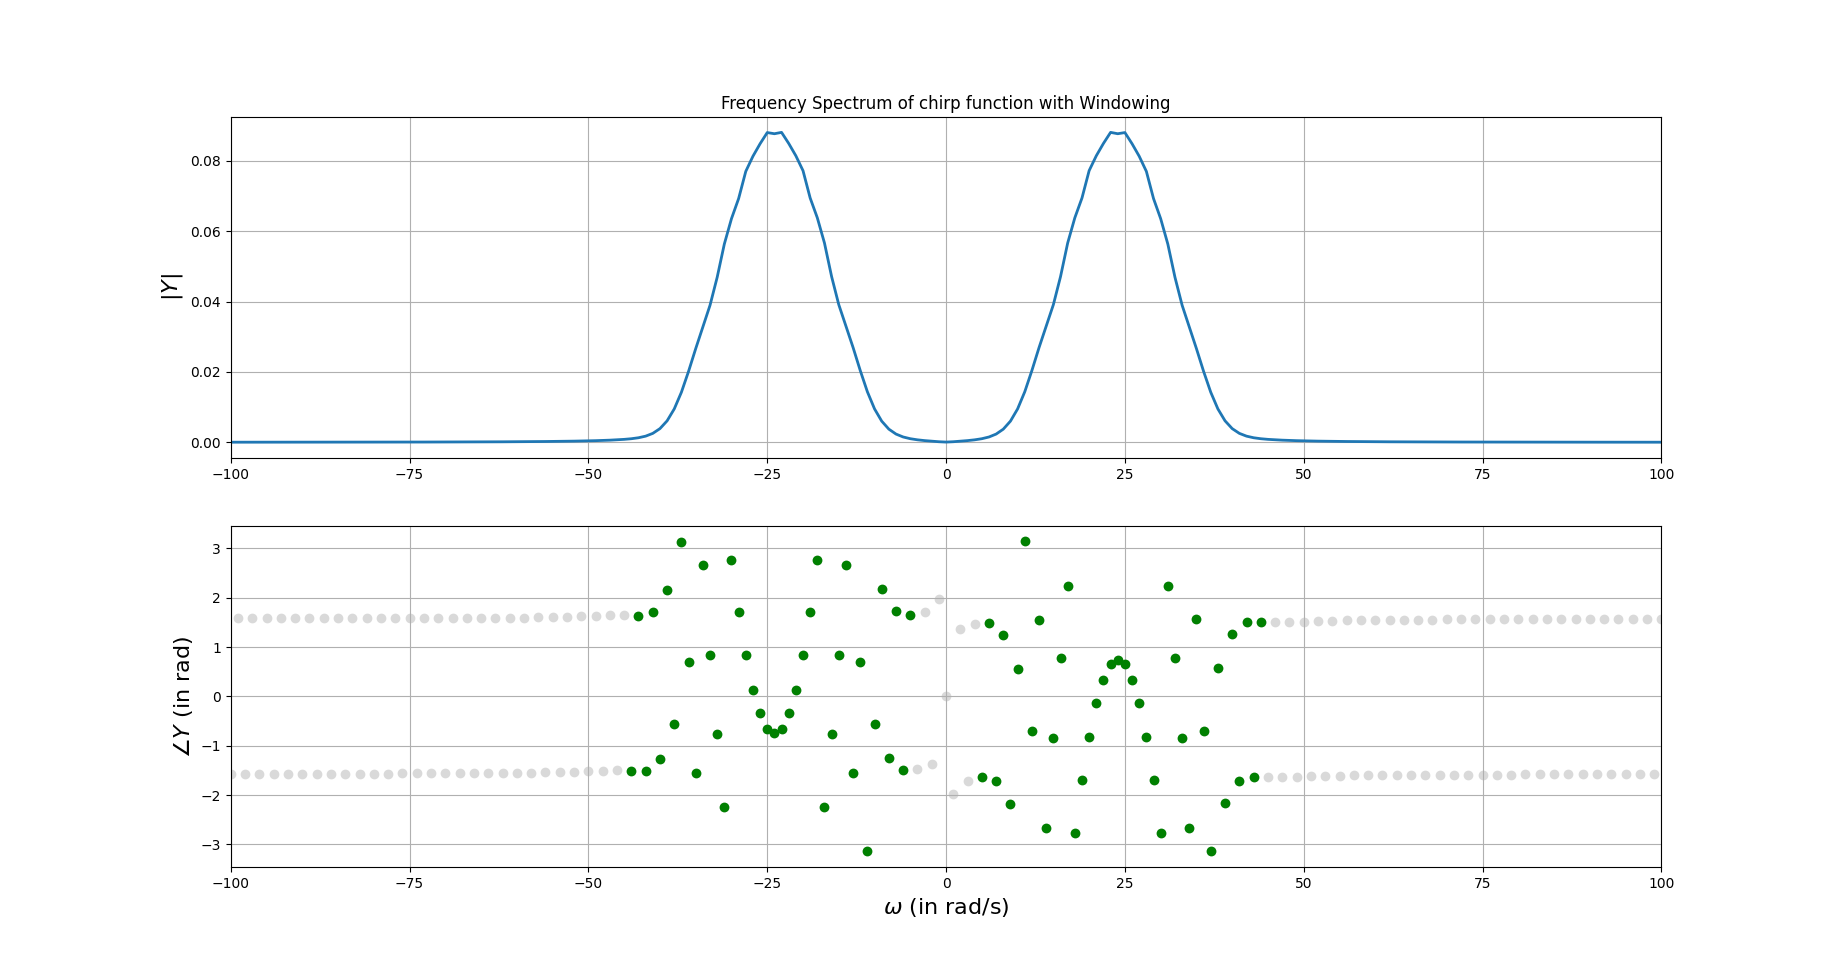
\includegraphics[scale=0.3]{Figure_5_2}}{\large\par}
\par\end{centering}
{\large{}\caption{{\large{}Frequency Spectrum of chirp function with Windowing}}
}{\large\par}
\end{figure}
{\large\par}
\noindent \begin{flushleft}
{\large{}There's a drastic change in the plot. This is because the
window function removed the discontinuities almost completely. This
is the advantage of Hamming Window. The main frequency of the signal
was isolated and made more easily identifiable by the window function.
In the case of chirped signal, the first term ($24t)$ is clearly
the more significant term and in the final plot we see the peak to
be at around 24. We also can expect the spectra to change with time
interval. We shall break 1024 samples from $[-\pi,\pi)$ into 16 contiguous
pieces of 64 samples each and find DFT for each interval.}{\large\par}
\par\end{flushleft}

{\large{}}
\begin{figure}[H]
\begin{centering}
{\large{}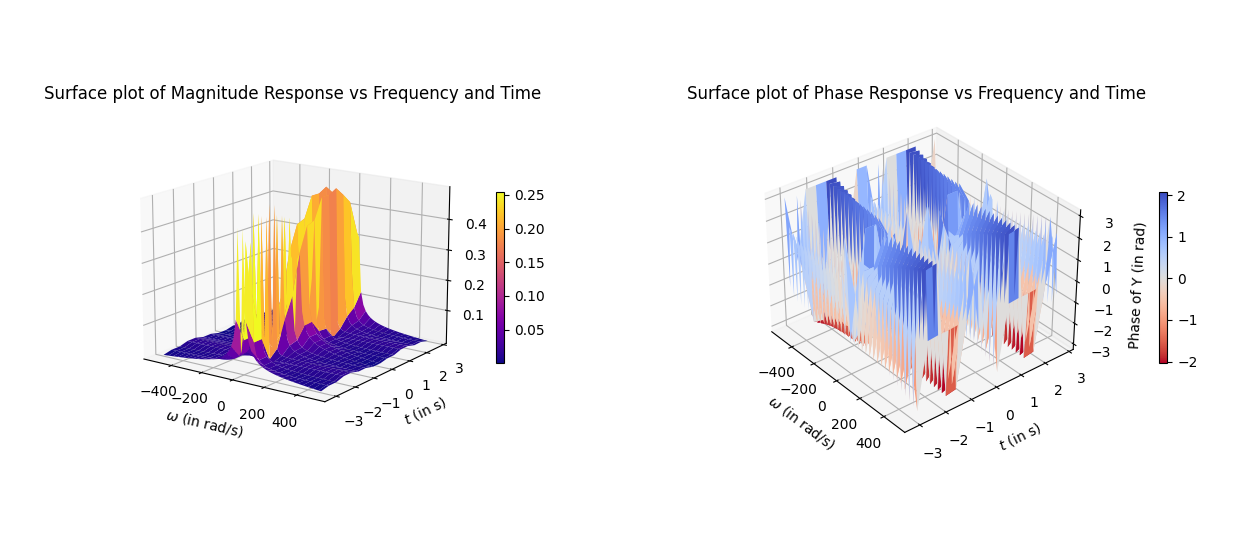
\includegraphics[scale=0.4]{Figure_6}}{\large\par}
\par\end{centering}
{\large{}\caption{{\large{}Frequency Spectra of chirped signal for different time ranges}}
}{\large\par}
\end{figure}
{\large\par}
\noindent \begin{flushleft}
{\large{}The gap between the peaks increases with time. Also the DFT
gets more well defined peaks with increasing time.}{\large\par}
\par\end{flushleft}

\section{Conclusion:}

{\large{}Thus, the Frequency Spectrum of some non-periodic signals
were analysed and plotted. We made use of Hamming Window and properties
of odd signals to reduce the errors which arise due to their non-periodic
nature. We also notice that Hamming Window increases the width of
the peaks slightly but more importantly it defines the peaks better.
We also extracted the frequency and phase shift using weighted average
method. We also analysed chirped signal at different time ranges and
understood their time variation of DFT.}{\large\par}
\end{document}
